%--------------------------------------------------------
%--------------------------------------------------------
%--------------------------------------------------------
%--------------------------------------------------------
\section{Introduction}
In late-stage lung cancer, airway narrowing (stenosis) due to tumor growth or compression affects approximately 30\% of patients, leading to severe respiratory distress, reduced quality of life, and increased mortality risk~\cite{Saji2010}. Accurate airway dimension measurements are critical for selecting appropriately sized stents to restore airway patency, a key palliative intervention. However, in advanced cases, conventional imaging like computed tomography (CT) often becomes unreliable due to tumor infiltration, mucus obstruction, or airway deformation. At our collaborating local hospital, clinicians rely on video bronchoscopy (VB) footage for intraoperative assessment, but they resort to subjective visual estimation of airway dimensions---a method prone to errors, especially under urgent conditions with poor image quality. This project explores software tools to provide objective, repeatable airway dimension estimates from VB footage, with the long-term aim of improving stent selection and patient outcomes.

The core challenge is to estimate real-world airway dimensions (in millimeters) from 2D VB images, which lack intrinsic scale references and suffer from wide-angle lens distortions, noise, and poor quality (e.g., blur from blood or mucus). This project leverages a known reference object, such as a biopsy forceps (probe) visible in the footage, to calibrate scale and infer the dimensions of stenotic airway cross-sections. An effective solution must be: (1) robust to the noisy, low-quality images common in late-stage lung cancer, (2) intuitive for clinicians to use during bronchoscopy, (3) capable of achieving sub-millimeter accuracy, and (4) validated against ground-truth measurements from controlled experiments or clinical data.

Current methods for airway dimension estimation primarily rely on CT-based modeling or intraoperative assessment. While CT is the gold standard, it often fails in advanced lung cancer due to obstructions or deformations~\cite{williamson2009}. VB offers real-time visualization but lacks scale, with studies reporting measurement errors up to 15.4\% due to lens distortion~\cite{Leigh2005}. Recent efforts, such as automated pipelines for subglottic stenosis estimation from VB footage~\cite{tomasini2025}, show promise but require traversing the stenosed region---an impractical step in severe cases. Other techniques, like anatomical optical coherence tomography (aOCT)~\cite{williamson2009}, provide high-resolution measurements but are limited to research settings due to specialized equipment needs. Thus, a practical, VB-based solution for advanced lung cancer remains an unmet need.

This project investigates a probe-based approach to estimate airway dimensions from VB footage, using a visible tool (e.g., biopsy forceps) as a scale reference. The work is currently in an early, experimental phase, focusing on proof-of-concept experiments and initial software prototypes to assess feasibility:
\begin{itemize}
    \item \textbf{Simplified 3D Tube Experiment}: A Blender-based simulation modeled the trachea as a hollow cylinder to test probe-based dimension estimation, achieving a mean error of 0.45~mm for circular cross-sections, with results and analysis detailed in subsequent sections.
    \item \textbf{Real Trachea Image CV Pipeline}: A computer vision pipeline was developed to detect C-shaped tracheal cartilages in real VB footage, using edge detection and ellipse fitting to approximate cross-sectional shapes.
    \item \textbf{Polygon Annotation App}: A PyQt5-based tool allows users to manually define arbitrary airway cross-sections via polygons and compute dimensions using probe calibration.
    \item \textbf{Virtual Probe App}: Another PyQt5-based tool enables interactive placement and scaling of a virtual probe for real-time dimension estimation.
\end{itemize}
These components represent initial steps toward addressing the challenges of poor image quality and distortions in late-stage lung cancer scenarios. While promising, the methods require further development and testing to determine their practical utility in clinical settings.

This exploratory work highlights the potential of probe-based dimension estimation for airway assessment in VB footage:
\begin{itemize}
    \item The simplified tube experiment achieved sub-millimeter accuracy (mean error: 0.45~mm) in a controlled environment, suggesting that, with refinement, the method might meet the precision needs for stent sizing.
    \item The CV pipeline identified tracheal cartilages in clear images, offering a possible foundation for semi-automated analysis in the future.
    \item The annotation tools provide intuitive manual calibration options, which could prove useful for handling noisy or distorted images.
\end{itemize}
These preliminary findings, derived from controlled experiments, indicate encouraging directions for future research. However, significant development and validation on clinical datasets are needed to transform these prototypes into a reliable, cost-effective, VB-based solution for cases where CT is unreliable, potentially enhancing stent selection and patient outcomes in complex clinical settings.

%--------------------------------------------------------
%--------------------------------------------------------
%--------------------------------------------------------
%--------------------------------------------------------

\section{Airway Narrowing in Late-Stage Lung Cancer}
Airway narrowing, medically termed stenosis, represents a significant and often debilitating complication in patients with late-stage lung disease, particularly those diagnosed with advanced lung cancer (Fig. \ref{fig:healty_vs_senosis}). This condition typically arises as malignant tumors grow into the airway lumen or exert external compression, leading to severe respiratory difficulties that profoundly impair patient quality of life. In advanced stages, airway obstruction can exacerbate symptoms and complicate therapeutic interventions, necessitating precise and timely management strategies.

\begin{figure}[h]
  \centering
  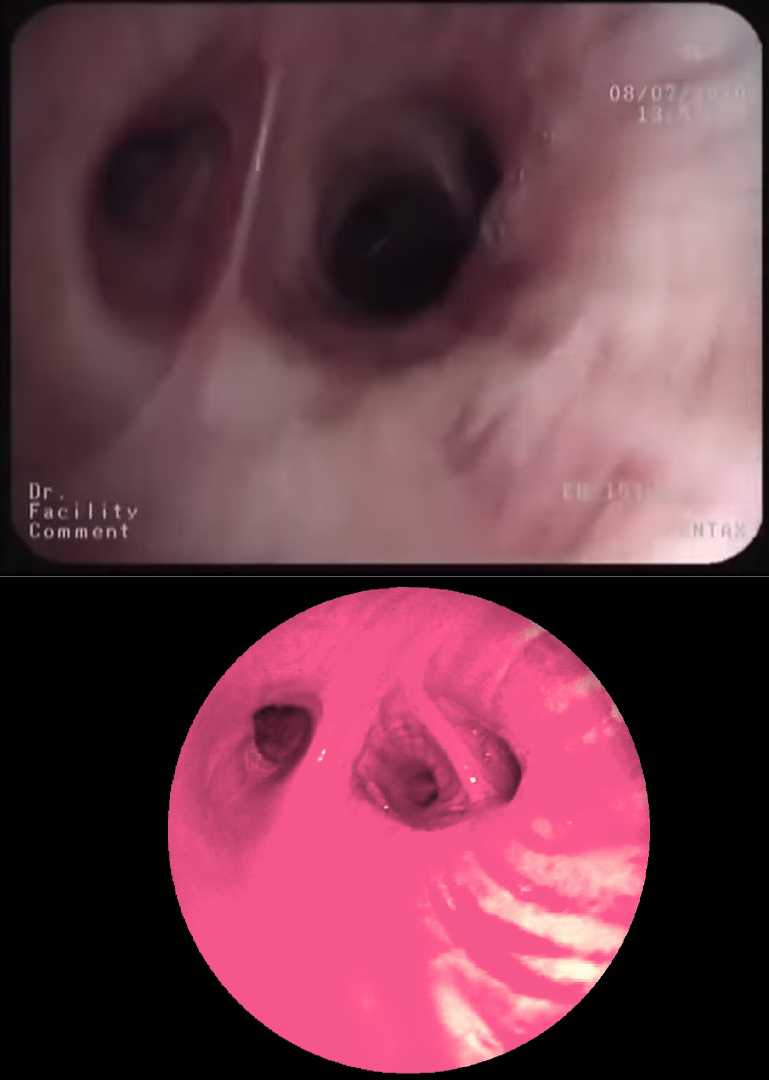
\includegraphics[width=0.49\textwidth]{images/02_med/healty_vs_senosis.png}
  \caption{Side-by-side comparison of a healthy airway (top) and a severely narrowed airway (bottom) in late-stage lung cancer. This visual contrast emphasizes the extent of stenosis and the importance of precise measurement for effective stent placement.}
  \label{fig:healty_vs_senosis}
\end{figure}

\subsection{Clinical Significance of Airway Narrowing}
The clinical ramifications of airway narrowing in late-stage lung cancer are substantial. Patients frequently present with dyspnea, stridor, and acute respiratory distress, which can escalate to life-threatening emergencies if untreated. Central airway obstruction is reported in 30\% of lung cancer cases, significantly contributing to morbidity and mortality~\cite{Saji2010}. Furthermore, airway stenosis can hinder the efficacy of systemic treatments such as chemotherapy or radiation by reducing patient respiratory capacity, underscoring the urgency of effective airway management.


\subsection{Treatment with Airway Stents}
Airway stents are a cornerstone of palliative care for airway narrowing in late-stage lung cancer. These devices, typically constructed from silicone or metal alloys, are deployed within the stenotic airway segment to restore patency and alleviate symptoms (Fig. \ref{fig:tracheal_bronchial_stent}). Placement is commonly performed via bronchoscopy, enabling direct visualization and precise positioning. However, the efficacy of stenting hinges on selecting an appropriately sized stent, a process contingent upon accurate measurement of the narrowed airway. Inaccurate sizing may precipitate complications, including stent migration, tissue overgrowth, or persistent obstruction.

\begin{figure}[h]
  \centering
  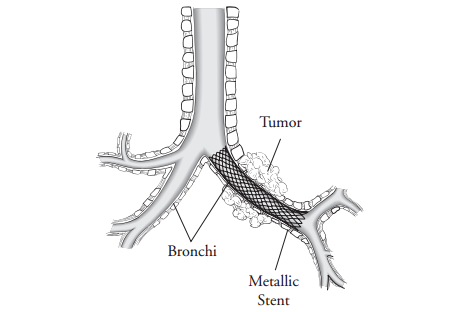
\includegraphics[width=0.49\textwidth]{images/02_med/tracheal_bronchial_stent.png}
  \caption{Diagram illustrating an airway stent deployed within a narrowed airway segment to maintain patency in a patient with tumor on Bronchi. Source: adapted from \cite{memorialsloan2025}}
  \label{fig:tracheal_bronchial_stent}
\end{figure}

\subsection{Challenges in Measuring Airway Dimensions}
Accurate airway dimension measurement is critical for successful stent placement, yet it poses significant challenges in late-stage lung cancer due to anatomical distortions and obstructions prevalent in advanced disease states.

\subsubsection{CT}
Computed Tomography (CT) remains the gold standard for airway assessment, offering detailed cross-sectional images to quantify the diameter and length of stenotic segments. However, its utility diminishes in severe cases where tumor infiltration, airway collapse, or mucus accumulation obscures boundaries, leading to measurement inaccuracies. Source: physicians at the local hospital.

\subsubsection{aOCT}
Anatomical Optical Coherence Tomography (aOCT) offers a high-resolution, real-time imaging solution for measuring airway dimensions during bronchoscopy, addressing limitations of conventional methods in late-stage lung cancer. Williamson et al. (2009) demonstrated aOCT's efficacy in four anesthetized patients, measuring airway dimensions from the trachea to subsegmental bronchi during bronchoscopy and comparing these with computed tomography (CT) measurements~\cite{williamson2009} (Fig. \ref{fig:aoct_vs_ct}). Their findings showed a close correlation between aOCT and CT, with aOCT reporting diameters and areas 7.6\% and 15.1\% higher, respectively, likely due to its sensitivity to dynamic airway features such as wall remodeling. However, aOCT's reliance on specialized equipment limits its widespread clinical adoption, confining its use primarily to research settings.

\begin{figure}[h]
  \centering
  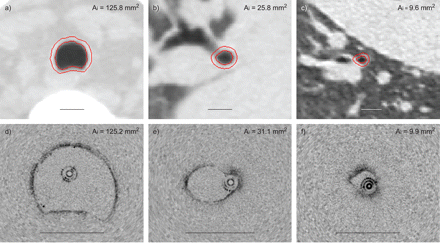
\includegraphics[width=1\columnwidth]{images/02_med/aoct_vs_ct.png}
  \caption{Computed tomography (CT) images (a–c) and their corresponding anatomical optical coherence tomography images (d–f) at: a) proximal trachea; b) left lower lobe; and c) medial segment of the right middle lobe bronchus. The CT images, taken at functional residual capacity, demonstrate the internal and external airway wall perimeter as calculated using Pulmonary Workstation 2.0 software (VIDA Diagnostics, Iowa City, IA, USA). Internal lumen area (Ai) measurements are shown for each technique. Scale bars=10mm. Source: adapted from ~\cite{williamson2009} }
  \label{fig:aoct_vs_ct}
\end{figure}


\subsubsection{VB}
Video Bronchoscopy (VB) facilitates direct, real-time airway visualization, offering dynamic insights into stenosis severity. However, VB lacks intrinsic scale references, rendering quantitative measurements subjective and error-prone. The wide-angle optics of bronchoscopes further introduce distortions, complicating dimensional accuracy (Fig. \ref{fig:vb_distortion}).

\begin{figure}[h]
  \centering
  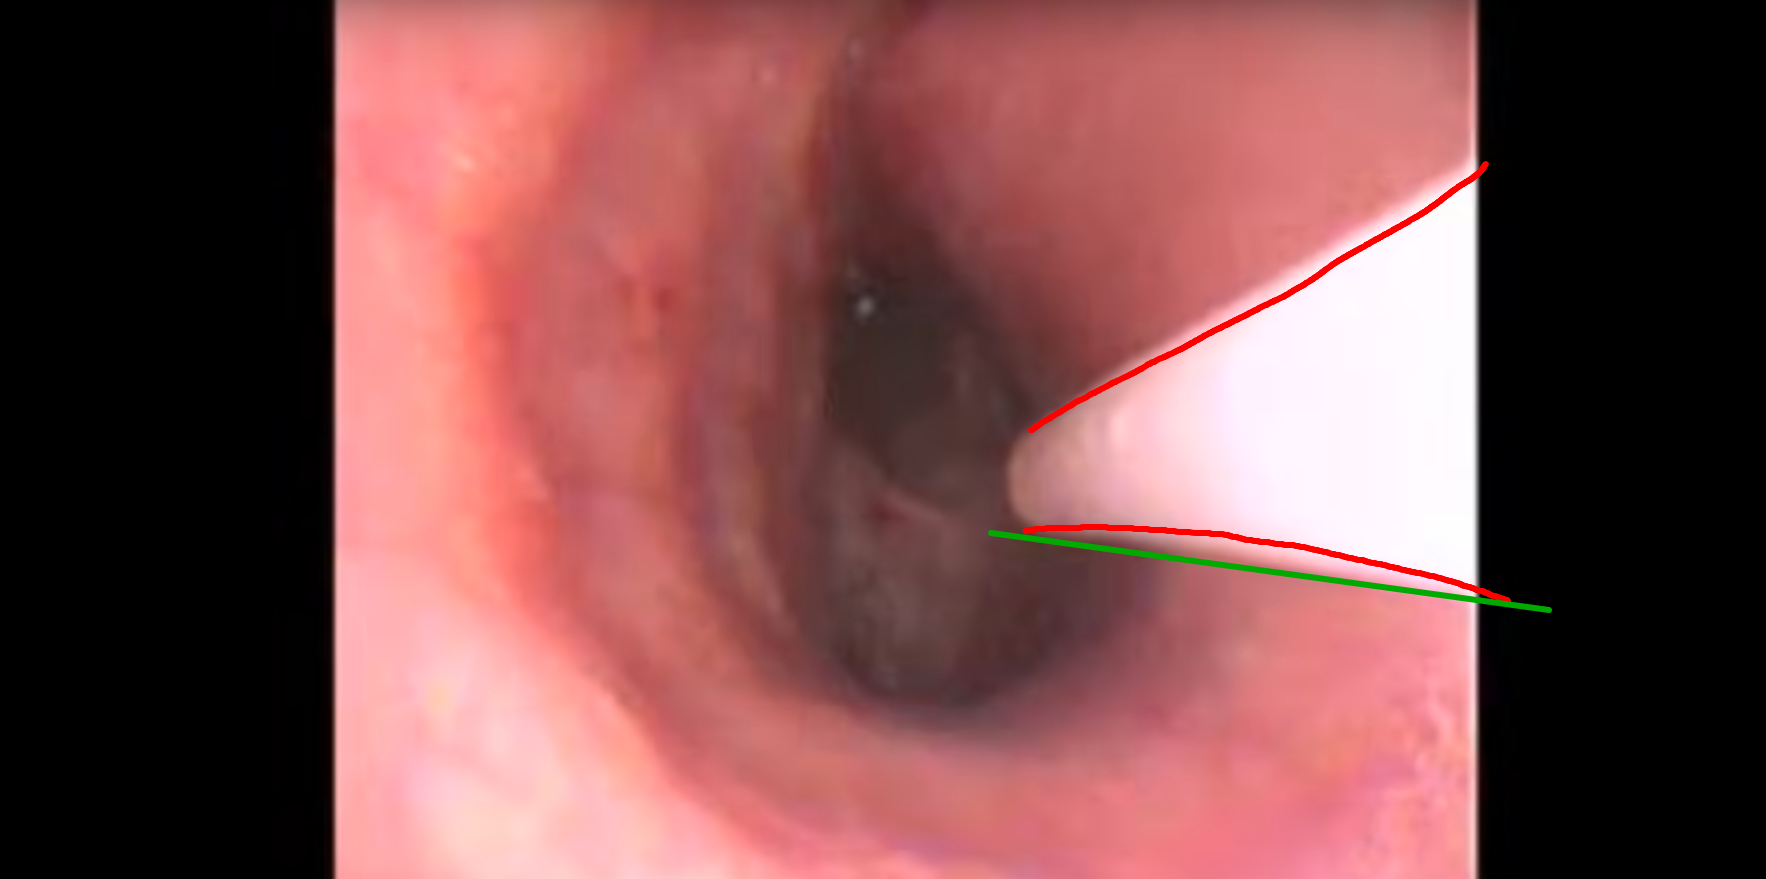
\includegraphics[width=1\columnwidth]{images/02_med/vb_distortion.png}
  \caption{A frame of VB (video bronchoscopy) showcasing optical distortions due to wide-angle lens. Red curve indicating the apparent shape of the tool. Green line for comparison.}
  \label{fig:vb_distortion}
\end{figure}

\section{VB for Stent Selection}
Video Bronchoscopy (VB) plays a pivotal role in airway stent selection for late-stage lung cancer, bridging diagnostic visualization with therapeutic intervention. This section explores its challenges, benefits, and contributions from recent literature, focusing on the last five referenced studies.

\subsection{Challenges and Benefits of VB}
Video bronchoscopy (VB)’s primary challenge lies in its inability to provide absolute scale references, necessitating reliance on visual estimation or external calibration tools. The wide-angle lens induces optical distortions, with studies reporting measurement errors, such as a 15.4\% reduction in magnification for a 6 mm object at 15 mm distance and up to 30\% geometric distortion at 3 mm without correction \cite{Leigh2005}. Conversely, VB’s benefits include real-time airway assessment, dynamic evaluation of obstruction under physiological conditions, and the capacity for immediate procedural adjustments during stent placement.

\subsection{Related work}
Numerous studies have addressed the challenge of quantifying airway dimensions using video bronchoscopy (VB), proposing methods to compensate for the lack of scale and the geometric distortions caused by endoscopic optics. These efforts span calibration-based approaches, image processing techniques, hardware integration, and more recently, automation through computer vision.

A foundational study by Doolin and Strande~\cite{doolin1995} introduced a physical calibration method using a standardized reference object. Their approach successfully reduced measurement errors from 17.6\% to 4.3\% in controlled environments, highlighting the importance of internal calibration when working with bronchoscopic video.

Expanding upon this idea, Santos et al.~\cite{santos1995} explored morphometric analysis for quantifying airway dimensions in bronchoscopy images. While their method yielded accurate results for airways with cross-sectional areas under 80~mm², its performance declined for larger regions, primarily due to distortion effects that were not adequately corrected.

Dorffel et al.~\cite{dorffel1999} proposed an integrated laser-probe system to assist VB measurements. This technique demonstrated high precision, achieving a correlation coefficient of 0.99 between estimated and ground-truth sizes in phantom and animal models. The results confirmed the potential of hardware augmented bronchoscopy for objective airway quantification.

Focusing on clinical reproducibility, Masters et al.~\cite{masters2005} developed a protocol tailored to pediatric airways, using flexible bronchoscopes. Their study reported high measurement consistency, with an intraclass correlation coefficient of 0.93. Although the target population was pediatric, the methodology is adaptable to broader clinical settings, including late-stage lung disease.

Czaja et al.~\cite{czaja2007} validated a quantitative VB technique on 40 adult patients by comparing measurements with CT-derived ground truths. Their results demonstrated excellent agreement, with a mean measurement deviation of only -0.071~mm. This provided a strong argument for the viability of VB as a diagnostic tool in adult patients where CT may not be feasible.

More recently, Tomasini et al.~\cite{tomasini2025} proposed a fully automated pipeline to estimate subglottic stenosis severity directly from bronchoscopy footage. Their method reconstructs a 3D model of the airway from a single frame using endoscopic illumination decline, bypassing the need to traverse the stenosed region. Their study reported strong agreement with both CT and expert annotations, and introduced the first public benchmark dataset in this domain. 

These studies collectively demonstrate VB’s evolution from a qualitative to a quantitative tool, with calibration and analytical methods enhancing its reliability for stent selection. Nonetheless, standardization across diverse patient populations and integration into routine workflows remain areas for further exploration.

%--------------------------------------------------------
%--------------------------------------------------------
%--------------------------------------------------------
%--------------------------------------------------------

\section{Hypothesis for Estimating Airway Dimensions}
Estimating the severity of airway stenosis from video bronchoscopy (VB) footage presents a significant challenge due to the absence of a scale reference. Without a known object for comparison, assessments of airway geometry lack a quantitative basis. To address this limitation, we propose the use of a rigid tool, such as biopsy forceps, inserted through the working channel of the bronchoscope and made visible in the footage. This tool functions as a probe, with known dimensions that can be extended or retracted, providing a scale reference for the airway structures captured in the image. While this approach could potentially be integrated with temporal data on bronchoscope head movement to construct an approximate 3D model based on light intensity variations, such a method would require high-quality footage. In our case, the reference VB footage, obtained from a patient with advanced lung cancer, exhibited significant occlusions, blood presence, and poor visibility in the lower airways. Consequently, tracking the camera head’s motion across multiple frames proved impractical, necessitating a method reliant on a single frame or a limited sequence of consecutive frames.

Our proposed solution imposes two critical prerequisites: (1) the probe must be positioned parallel to the airway wall, ensuring alignment with its contour, and (2) the probe’s tip must be located at the same distance from the camera as the airway cross-section under evaluation, or in contact with it. These conditions minimize perspective-induced distortions, particularly for circular or elliptical shapes, which could otherwise skew dimensional estimates due to unknown camera angles.

However, the inherent limitations of VB footage must be acknowledged. Poor image sharpness, primarily resulting from the subtle movement of the bronchoscope head, which is challenging to stabilize at such a fine scale, and obstructions from blood or mucus that either directly obscure the camera lens or interfere with its autofocus mechanism, significantly degrades image quality. These factors obscure fine details, particularly within the central 30\% of the image. Consequently, our method is designed to provide an approximate estimation of airway dimensions rather than a precise measurement. These constraints reflect the challenging clinical conditions under which the footage is acquired, underscoring the need for alternative approaches to enhance utility despite suboptimal data quality.

Given these considerations, we adopted an incremental strategy, initiating our investigation with simplified experiments. The trachea, characterized by its relatively uncomplicated tubular geometry, was selected as the starting point for this exploratory work.

\section{Simplified 3D Tube Experiment}

To assess the feasibility of our probe-based estimation method, I conducted a controlled experiment using a simplified 3D model of the trachea. The trachea was represented as a hollow cylinder, constructed within Blender, a 3D modeling software. A virtual camera was positioned inside the cylinder, with a cylindrical probe attached to it, replicating the configuration of a bronchoscopy tool. To reduce optical distortions in this preliminary test, the camera was assigned a field of view (FOV) of approximately 66.8°, a value selected to balance visibility and accuracy.

\subsection{Experimental Setup}

The tracheal model was generated by applying a Boolean subtraction operation between two cylinders, with the smaller cylinder defining the inner diameter of the tube. The model was centered in the scene along the x, y, and z axes, with the z-axis oriented vertically to reflect the anatomical alignment of the human trachea. This orientation facilitated precise camera placement and ensured that the probe could be aligned parallel to the tube wall, while also enabling intuitive navigation within the 3D environment.

The virtual camera was configured with a vertical sensor fit, a sensor height of 3.63 mm, and a focal length of 2.75 mm, parameters consistent with those of a real-world Raspberry Pi camera module. This configuration produced an FOV of 66.8°, and the rendered images were output at a resolution of 3,280 × 2,464 pixels.

The probe, modeled as a cylinder with a diameter of 2 mm and a length of 25 mm to represent biopsy forceps, was parented to the camera. This ensured that the probe moved in tandem with the camera, maintaining a fixed relative position offset by -6 mm on the x-axis and 0 mm on the y-axis.

Using this setup, I rendered four sets of five images each, varying the inner diameter of the tube across the sets: 14 mm, 17 mm, 21 mm, and 28 mm. For each diameter, the camera was positioned at five distinct distances along the tube’s length, as depicted in Figure \ref{fig:sim_cam_pos_comparison}. This approach generated a series of images in which the probe’s position remained constant, while the size and position of the circular cross-section at the tube’s end varied systematically.

\begin{figure}[h]
  \centering
  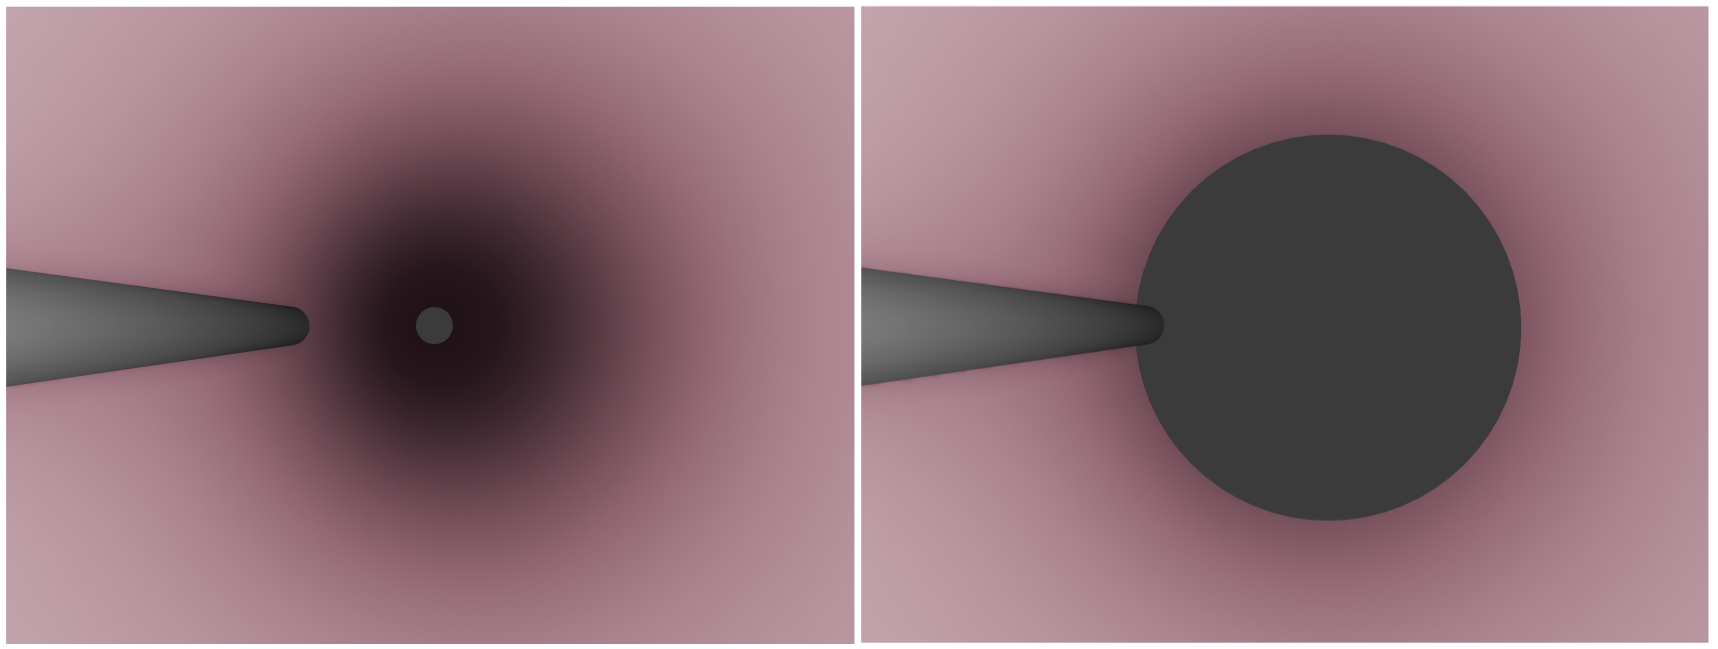
\includegraphics[width=1\columnwidth]{images/05_tube/sim_cam_pos_comparison.png}
  \caption{Side-by-side comparison of renders with the camera positioned at the first distance category (left) and the fifth distance category (right). The inner diameter of the tube is 21 mm in both images.}
  \label{fig:sim_cam_pos_comparison}
\end{figure}

\subsection{Probe Localization in the Image}
\label{sec:FindingTheProbe}

To correlate the probe’s 3D position with its 2D appearance in the rendered images, I manually annotated the pixel positions and sizes of the probe’s base and tip across a range of configurations. Specifically, I collected metadata for probe extensions of +0.5 mm, +1.0 mm, +1.5 mm, -0.5 mm, -1.0 mm, -1.5 mm, and -1.6 mm along the z-axis, simulating varying degrees of extrusion from the bronchoscopy head. The annotated features included the x and y coordinates of the probe tip’s center and its radius in pixels.

When these features were plotted against the probe length (defined as the distance from the camera to the probe tip), most exhibited a linear relationship. However, the x-coordinate of the probe tip’s center displayed a logarithmic trend, as illustrated in Figure \ref{fig:probe_lenght_vs_features}.

\begin{figure}[h]
  \centering
  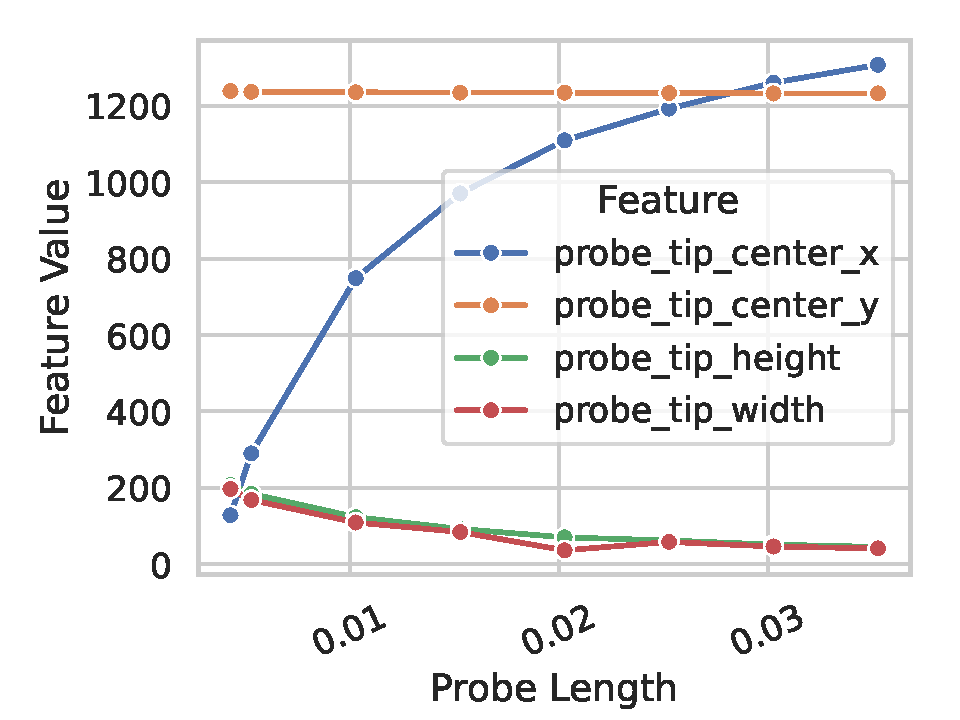
\includegraphics[width=1\columnwidth]{images/05_tube/probe_length_vs_features.pdf}
  \caption{Plot of the measured pixel values for the probe tip’s center x-coordinate, center y-coordinate, and radius against the probe length (distance from the camera to the probe tip in the 3D scene).}
  \label{fig:probe_lenght_vs_features}
\end{figure}

\subsubsection{Metadata Processing}
\label{sec:ProcTheMeta}

The annotated metadata was utilized to derive two fitting functions characterizing the relationship between the probe’s appearance in the image and its physical dimensions. The first function, an exponential model, describes the relationship between the x-coordinate of the probe tip’s left center point (in pixels) and the probe’s actual length (in millimeters), as shown in Figure \ref{fig:curve_fits_probe_tip_left_x_to_length}. The second function, a linear model, relates the same x-coordinate to the probe tip’s apparent radius (in pixels), as illustrated in Figure \ref{fig:curve_fits_probe_tip_left_x_to_height}. These functions are highly dependent on the probe’s 3D position, the camera’s field of view (FOV), and the image resolution. While this dependency limits their generalizability, the functions were sufficient for the controlled conditions of this experiment and provided a foundation for subsequent image analysis.

\begin{figure}[h]
  \centering
  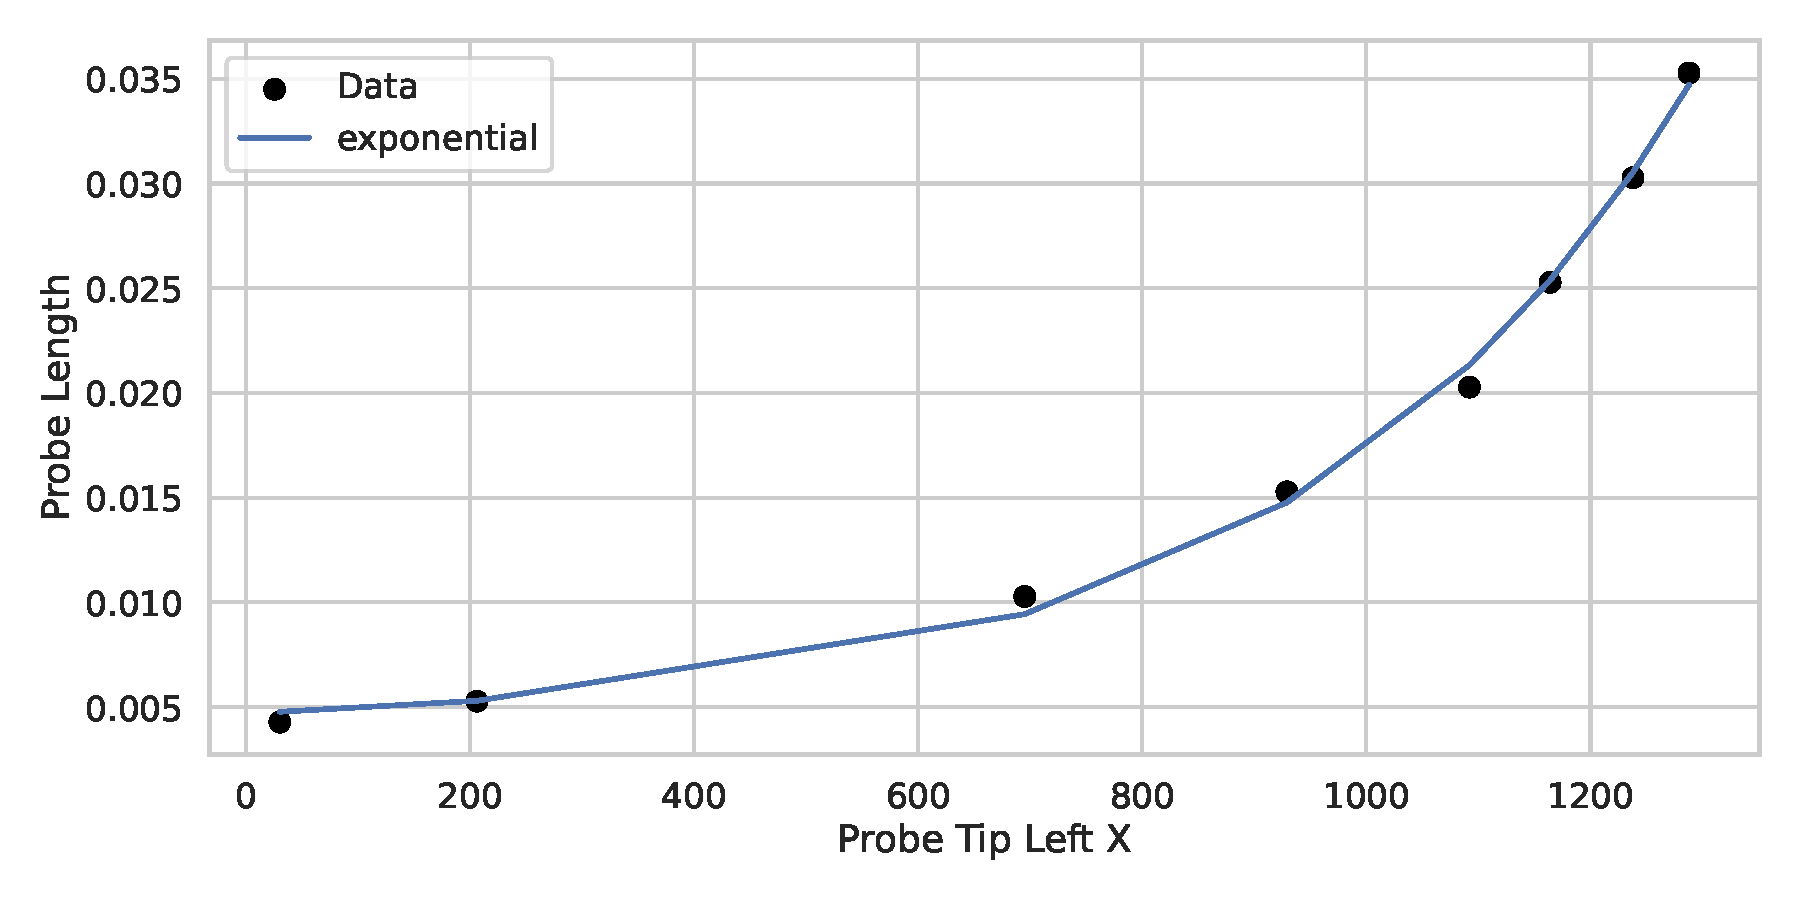
\includegraphics[width=1\columnwidth]{images/05_tube/curve_fits_probe_tip_left_x_to_length.pdf}
  \caption{Plot of an exponential function fitted to data, representing the relationship between the x-coordinate of the probe tip’s left center point (probe\_tip\_left\_x) and the probe length (in millimeters).}
  \label{fig:curve_fits_probe_tip_left_x_to_length}
\end{figure}

\begin{figure}[h]
  \centering
  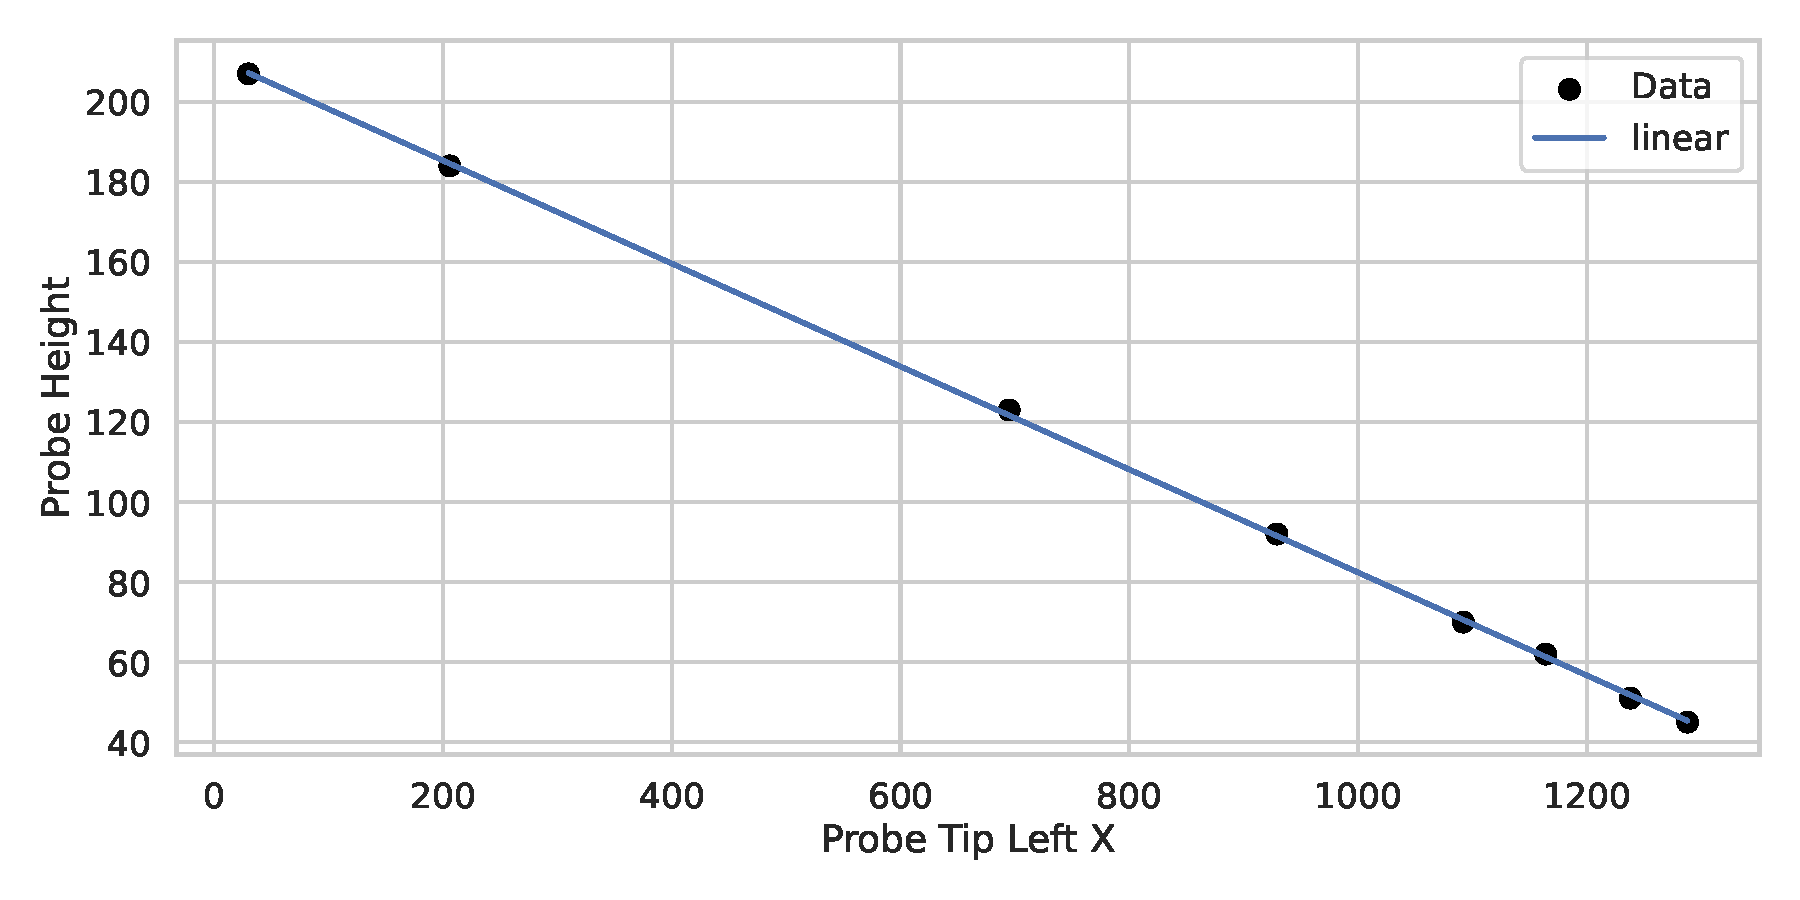
\includegraphics[width=1\columnwidth]{images/05_tube/curve_fits_probe_tip_left_x_to_height.pdf}
  \caption{Plot of a linear function fitted to data, representing the relationship between the x-coordinate of the probe tip’s left center point (probe\_tip\_left\_x) and the probe tip’s radius (in pixels).}
  \label{fig:curve_fits_probe_tip_left_x_to_height}
\end{figure}

\subsection{Metadata-Aided Semi-Automated Image Analysis}
\label{sec:cv_meta_analysis}

The objective of this experiment was to estimate the dimensions of a shape located at an arbitrary distance from the probe tip, under the condition that the shape lies at the end of a wall parallel to the probe. This setup assumes that extending the probe would bring its tip into contact with the shape’s perimeter. Successfully estimating dimensions for a simple circular shape would establish a proof-of-concept, with the potential to extend the method to more complex geometries by accurately identifying their perimeter and position within the image.

The dimension estimation process comprises the following steps:
\begin{enumerate}
    \item \textbf{Shape Detection.} For the generated images containing circular cross-sections, the target shape was identified using circle detection methods from the OpenCV Python library, as indicated by the green circle in Figure \ref{fig:sim_annotated}.
    \item \textbf{Probe Localization.} The positions of the probe’s base and tip were predefined as constants in the code, based on the manually collected metadata (labeled as \texttt{a} and \texttt{c}, respectively, in Figure \ref{fig:sim_annotated}).
    \item \textbf{Probe Direction Vector.} The probe’s direction vector was calculated by subtracting the probe tip’s center position from the base’s center position and normalizing the result.
    \item \textbf{Probe Tip Left Position.} The x-coordinate of the probe tip’s left position was computed as the x-coordinate of the probe tip’s center minus its radius (in pixels), with the y-coordinate identical to that of the probe tip’s center (labeled as \texttt{b} in Figure \ref{fig:sim_annotated}).
    \item \textbf{Intersection Calculation.} The intersection between a line defined by the probe’s direction vector (originating at the probe tip’s left position) and the detected circle was computed using standard geometric methods. If two intersection points were identified, the one closer to the probe tip was selected (labeled as \texttt{d} in Figure \ref{fig:sim_annotated}).
    \item \textbf{Scale Ratio Determination.} The prediction function from Section \ref{sec:ProcTheMeta} was used to estimate the probe’s radius (in pixels) at the given distance. This value was divided by the known probe radius (in millimeters) to compute a pixel-to-millimeter scale ratio.
    \item \textbf{Dimension Estimation.} The detected circle’s radius (in pixels) was multiplied by the pixel-to-millimeter scale ratio to estimate the shape’s diameter in millimeters.
\end{enumerate}

\begin{figure}[h]
  \centering
  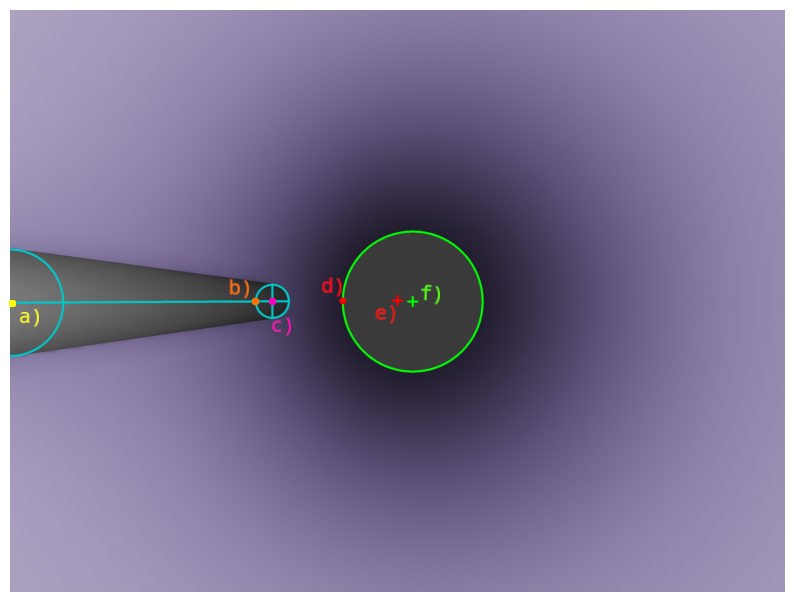
\includegraphics[width=1\columnwidth]{images/05_tube/sim_annotated.png}
  \caption{Annotated image depicting the probe-camera configuration at the third distance category, within a tube of 21 mm inner diameter. Labels indicate: \textbf{a)} probe base center, \textbf{b)} probe tip left, \textbf{c)} probe tip center, \textbf{d)} intersection of the probe vector (from point \texttt{b}) with the green circle (target shape), \textbf{e)} image center, \textbf{f)} center of the green circle.}
  \label{fig:sim_annotated}
\end{figure}

\subsection{Results}

The estimation process was applied to all 20 generated images, organized in a data frame to evaluate the method’s accuracy. A scatter plot of predicted versus actual tube inner radii (Figure \ref{fig:predicted_vs_real_radius}) demonstrates that the predictions closely align with the ideal prediction line, indicating promising accuracy under controlled conditions.

\begin{figure}[h]
  \centering
  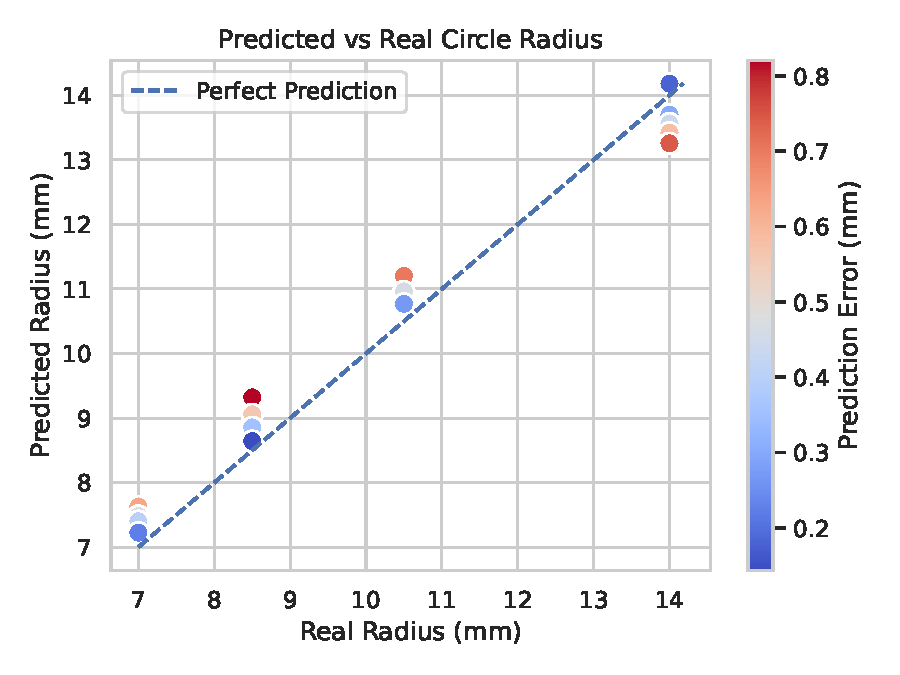
\includegraphics[width=1\columnwidth]{images/05_tube/predicted_vs_real_radius.pdf}
  \caption{Scatter plot comparing actual tube inner radii (x-axis) with predicted radii (y-axis), with the ideal prediction line included.}
  \label{fig:predicted_vs_real_radius}
\end{figure}

A heatmap of prediction errors (Figure \ref{fig:heatmap_prediction_error}) reveals that errors were greatest in the first distance category, where the camera was farthest from the tube’s end. This aligns with the expectation that a smaller, more distant target shape reduces the number of pixels available for accurate intersection calculations, thereby increasing error. Notably, the 14 mm radius exhibited an inverse error trend across distance categories compared to smaller radii, suggesting potential sensitivity to larger shapes.

\begin{figure}[h]
  \centering
  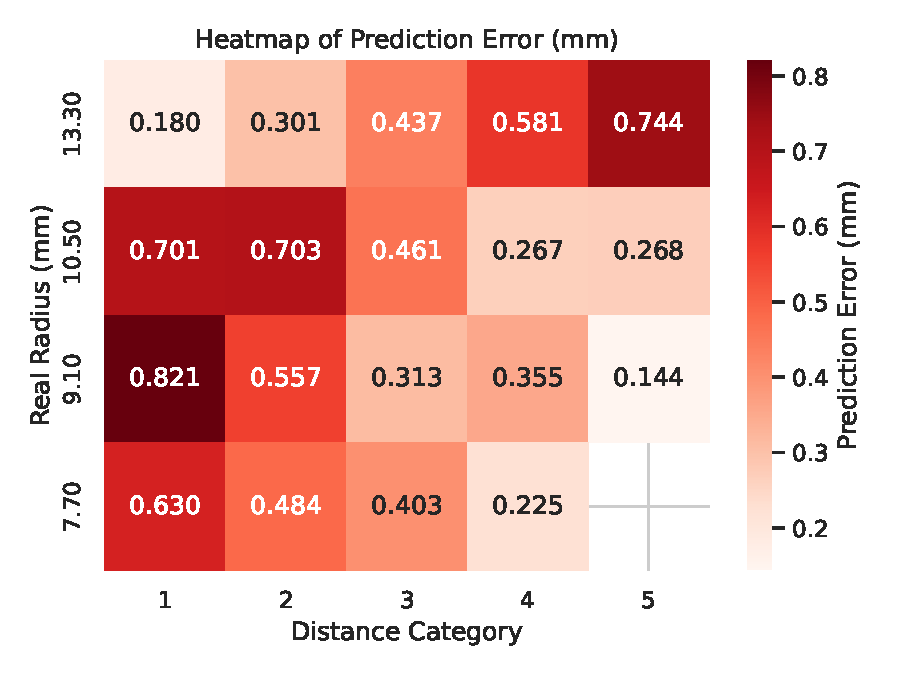
\includegraphics[width=1\columnwidth]{images/05_tube/heatmap_prediction_error.pdf}
  \caption{Heatmap of prediction errors (in millimeters), with distance category (x-axis) and actual radius (y-axis). Error magnitude is indicated by the intensity of the red color.}
  \label{fig:heatmap_prediction_error}
\end{figure}

Box plots of errors grouped by actual radius (Figure \ref{fig:box_plot_prediction_error}) show no distinct pattern across groups, suggesting consistent performance regardless of tube size, a positive indicator of robustness.

\begin{figure}[h]
  \centering
  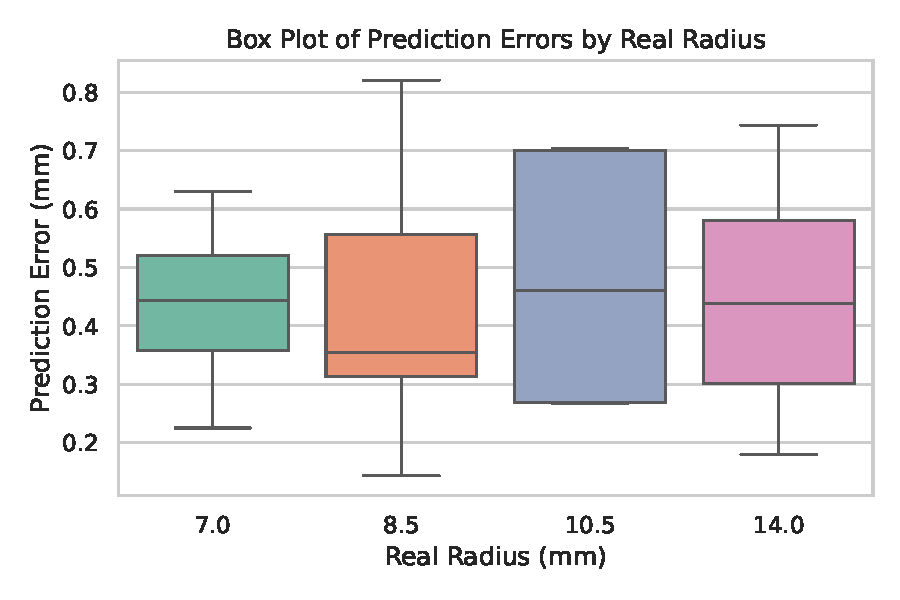
\includegraphics[width=1\columnwidth]{images/05_tube/box_plot_prediction_error.pdf}
  \caption{Box plots illustrating the magnitude of prediction errors, grouped by actual tube inner radius.}
  \label{fig:box_plot_prediction_error}
\end{figure}

Conversely, box plots grouped by distance category (Figure \ref{fig:box_plot_prediction_error_by_distance}) confirm a clear trend: mean error decreases as the camera approaches the tube’s end, corroborating the heatmap findings.

\begin{figure}[h]
  \centering
  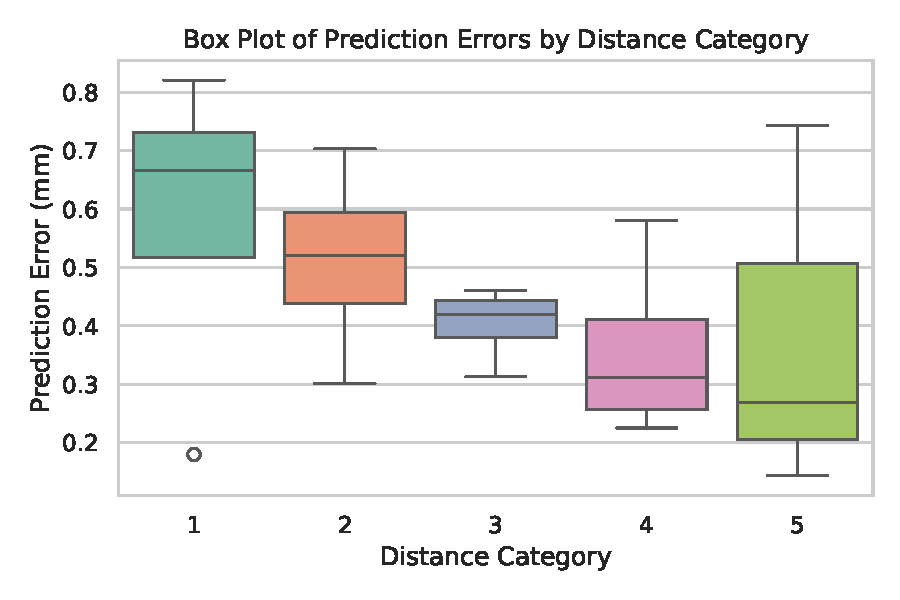
\includegraphics[width=1\columnwidth]{images/05_tube/box_plot_prediction_error_by_distance.pdf}
  \caption{Box plots illustrating the magnitude of prediction errors, grouped by distance category (distance from camera to tube end in millimeters).}
  \label{fig:box_plot_prediction_error_by_distance}
\end{figure}

A violin plot of the error distribution across the dataset (Figure \ref{fig:violin_plot_all_prediction_errors}) indicates that most errors fall between 0.28 mm and 0.61 mm, reflecting a concentrated range of variability.

\begin{figure}[h]
  \centering
  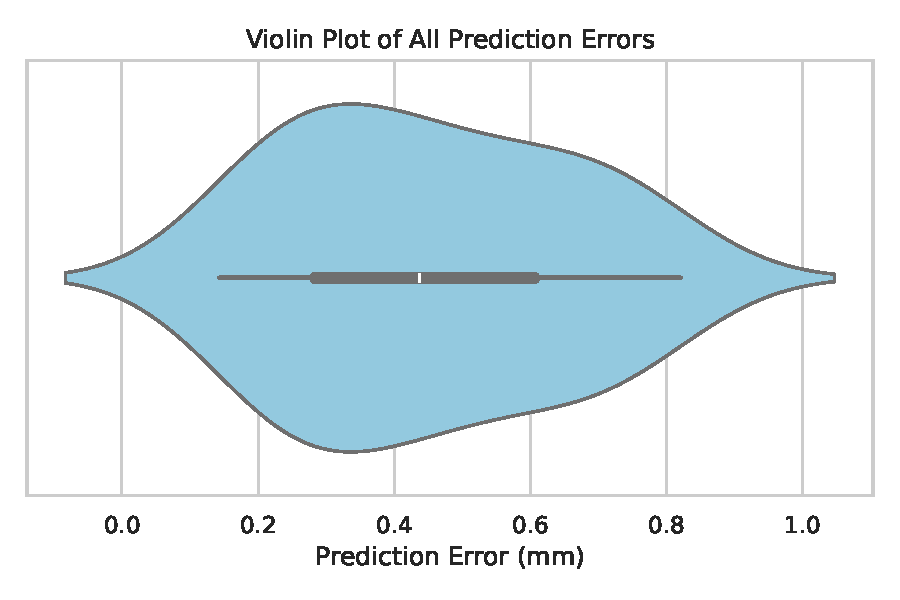
\includegraphics[width=1\columnwidth]{images/05_tube/violin_plot_all_prediction_errors.pdf}
  \caption{Violin plot depicting the distribution of prediction error magnitudes across the dataset.}
  \label{fig:violin_plot_all_prediction_errors}
\end{figure}

Statistical analysis of the errors yields a mean of 0.451 mm, a minimum of 0.144 mm, and a maximum of 0.821 mm, as summarized in Table \ref{tab:prediction_errors}.

\begin{table}[h]
\centering
\caption{Statistical Summary of Prediction Errors (mm)}
\begin{tabular}{lr}
\toprule
Statistic & Value (mm) \\
\midrule
Mean & 0.451 \\
Standard Deviation & 0.204 \\
Minimum & 0.144 \\
25th Percentile & 0.285 \\
Median (50th Percentile) & 0.437 \\
75th Percentile & 0.605 \\
Maximum & 0.821 \\
\bottomrule
\end{tabular}
\label{tab:prediction_errors}
\end{table}

\subsection{Potential Improvements and Conclusion}

To enhance this method, future work could programmatically replicate the Blender scene to dynamically compute pixel-to-millimeter ratios, eliminating reliance on empirically derived fitting functions and improving generalizability.

\subsubsection{Potential Extensions}
Further development could explore the following:
\begin{enumerate}
    \item Generating datasets with varied fields of view to assess robustness across imaging conditions.
    \item Implementing corrections for optical lens distortions, which are prevalent in real bronchoscopy systems.
    \item Extending the method to non-circular airway cross-sections, such as ellipses or irregular shapes.
    \item Evaluating the impact of varying probe sizes and positions on estimation accuracy.
    \item Accounting for the non-uniform, non-cylindrical nature of real tracheal walls, which may introduce additional complexities.
\end{enumerate}

\subsubsection{Conclusion}

Analysis of the 20-image dataset suggests that the proposed method offers a promising approach for estimating tube cross-sectional dimensions from a single image in a controlled environment. All predictions were within 1 mm of the actual values, with a maximum error of 0.821 mm and a median error of 0.437 mm. However, these results were obtained under simplified conditions, with a low FOV and idealized geometry. For practical application, factors such as high-FOV distortions, variable lighting, and poor image quality due to clinical conditions must be addressed. These preliminary findings provide a foundation for further refinement, highlighting the potential of probe-based estimation for airway dimension measurement.

%--------------------------------------------------------
%--------------------------------------------------------
%--------------------------------------------------------
%--------------------------------------------------------

\section{Trachea Dimension Estimation via Computer Vision Pipeline}

To extend the findings from the simplified tube experiment, this study explored a more anatomically representative approach by focusing on the trachea’s C-shaped cartilaginous rings. These structures, when viewed in cross-section, serve as distinct anatomical landmarks that facilitate the identification of airway geometry. Accurate detection of these tracheal cartilages could also enable estimation of the camera’s rotational orientation within the trachea, as the rings appear asymmetrically distributed in the image due to perspective effects.

\subsection{Dynamic 3D Trachea Model}

Motivated by the need for a more realistic tracheal representation, a dynamic, scalable 3D model was developed using Blender. The model was constructed by defining a sinusoidal profile to represent the depth variations of the tracheal cartilages, which was then extruded to form a vase-like structure. To approximate the trachea’s elliptical cross-section, the model was scaled along the x-axis. A rectangular prism was incorporated along one of the narrower walls to simulate a structural feature interacting with the cartilages, as shown in Figure \ref{fig:trachea_model}. The camera and probe configuration from the prior tube experiment was reused, with the probe positioned such that its tip contacted one of the C-shaped cartilages. The scene was rendered at a resolution of 3,280 × 2,464 pixels, consistent with previous experiments.

\begin{figure}[h]
  \centering
  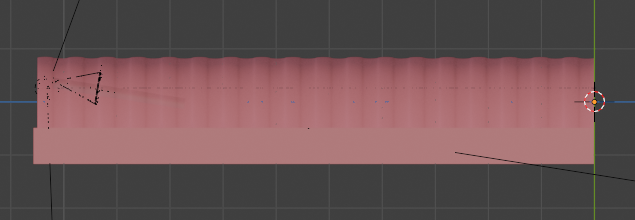
\includegraphics[width=1\columnwidth]{images/06_trach_cv/trachea_model.png}
  \caption{Side-view screenshot of a simplified 3D trachea model, highlighting the distinct C-shaped cartilaginous rings.}
  \label{fig:trachea_model}
\end{figure}

A computer vision (CV) pipeline was developed to detect the simulated cartilages in the rendered images. While the pipeline successfully delineated the cartilage boundaries, its performance was heavily influenced by lighting artifacts, particularly the shadows cast by the cartilaginous structures, as illustrated in Figure \ref{fig:sim_trachea_contour}. Attempts to mitigate these shadows through varied lighting configurations were unsuccessful, indicating a dependency on rendering conditions. To address this limitation and evaluate the pipeline under more realistic conditions, a real bronchoscopy image was sourced for further analysis.

\begin{figure}[h]
  \centering
  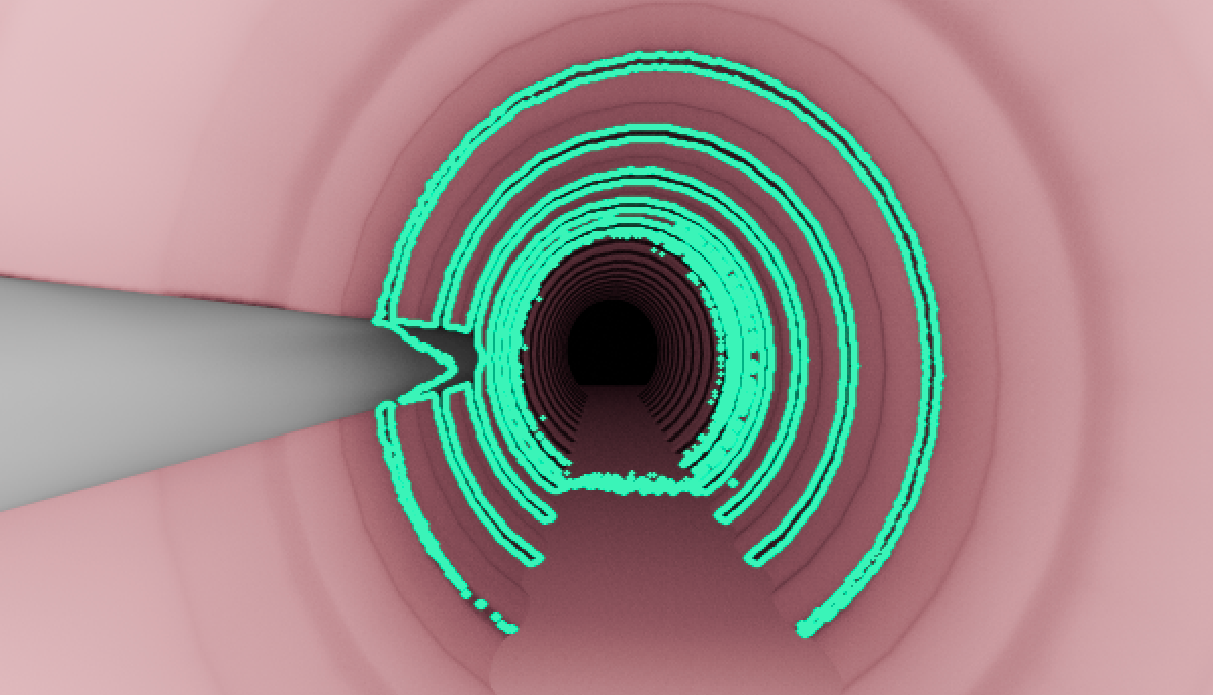
\includegraphics[width=1\columnwidth]{images/06_trach_cv/sim_trachea_cotour.png}
  \caption{Render of the trachea model with cartilage boundaries highlighted by the CV pipeline, primarily due to shadows cast by the cartilaginous rings.}
  \label{fig:sim_trachea_contour}
\end{figure}

\subsection{Application to Real Trachea Image}

To test the CV pipeline on clinical data, a publicly available VB image was selected, depicting the trachea with the camera approximately parallel to the airway wall \cite{VUUniversityMedicalCenterAmsterdam2025}. This image was chosen for its clarity and relevance to the study’s objectives.

The image processing pipeline, outlined in Figure \ref{fig:image_processing_grid}, comprises the following steps to detect C-shaped tracheal cartilages:

\begin{enumerate}
    \item \textbf{Source Image}: The input is an original VB frame capturing the trachea, displaying C-shaped cartilages and surrounding mucosal tissue.
    \item \textbf{Bilateral Filtering}: Noise is reduced while preserving cartilage edges using a bilateral filter with a diameter $d=3$, color standard deviation $\sigma_{\text{Color}} = 150$, and spatial standard deviation $\sigma_{\text{Space}} = 75$.
    \item \textbf{Median Blur Filtering}: Small artifacts, such as salt-and-pepper noise, are eliminated using a $5 \times 5$ pixel kernel, enhancing cartilage boundaries.
    \item \textbf{Image Sharpening}: Cartilage edges are accentuated with a $3 \times 3$ sharpening kernel, improving edge detection accuracy.
    \item \textbf{Canny Edge Detection}: Cartilage boundaries are identified in the grayscale image following a $5 \times 5$ Gaussian blur (standard deviation $\sigma = 0$), with thresholds $T_1 = 50$ and $T_2 = 150$ and an aperture size of 3.
    \item \textbf{Gaussian Blur Smoothing}: The edge-detected image is smoothed to reduce false edges, applying a Gaussian blur with a $9 \times 9$ kernel.
    \item \textbf{Binary Thresholding}: Cartilage regions are isolated using a binary threshold of 100 (maximum value 255), generating a binary image.
    \item \textbf{Contour Detection}: Closed shapes in the binary image are identified as potential cartilage outlines.
    \item \textbf{Closest Contour Selection}: The contour nearest to the probe’s right edge is selected as the C-shaped cartilage, determined by minimizing the absolute distance via point-to-polygon testing.
    \item \textbf{Ellipse Fitting}: An ellipse is fitted to the selected contour to approximate the cross-sectional shape of the airway.
\end{enumerate}

\begin{figure}[h]
\centering
\begin{minipage}[t]{0.48\columnwidth} % Left column
    \centering
    \begin{tikzpicture}
        \node[anchor=south west,inner sep=0] (image) at (0,0) {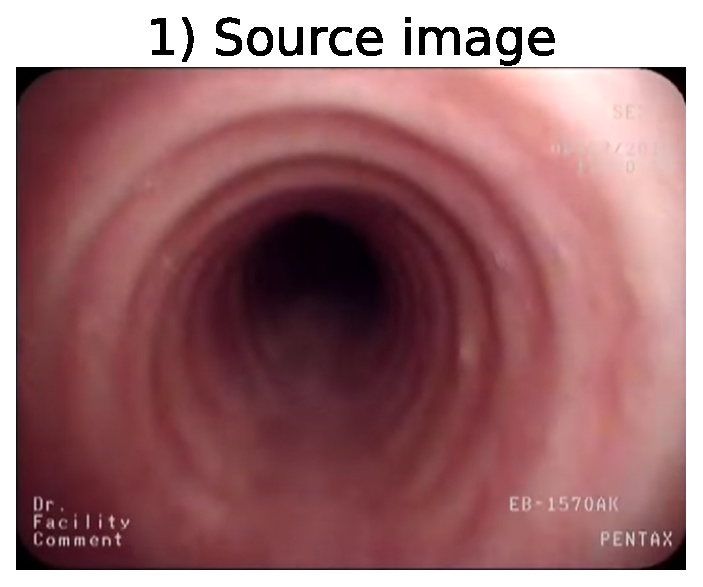
\includegraphics[width=\textwidth]{images/06_trach_cv/01_source_image.pdf}};
    \end{tikzpicture}
    \begin{tikzpicture}
        \node[anchor=south west,inner sep=0] (image) at (0,0) {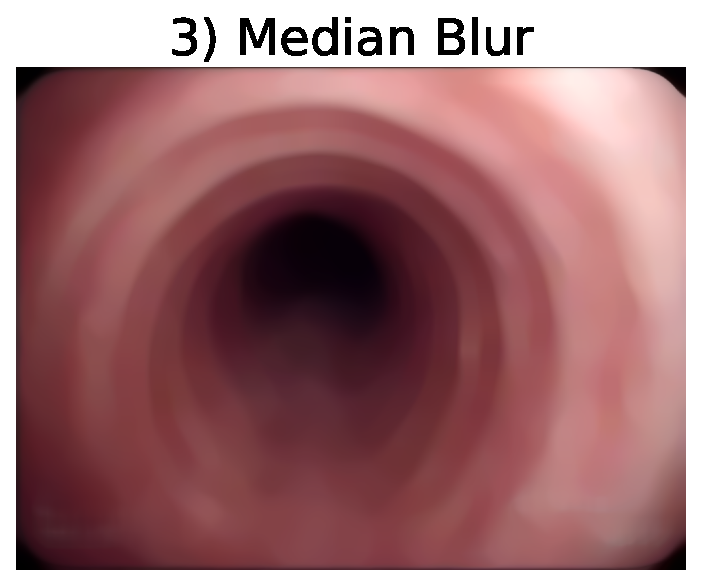
\includegraphics[width=\textwidth]{images/06_trach_cv/03_median_blur.pdf}};
    \end{tikzpicture}
    \begin{tikzpicture}
        \node[anchor=south west,inner sep=0] (image) at (0,0) {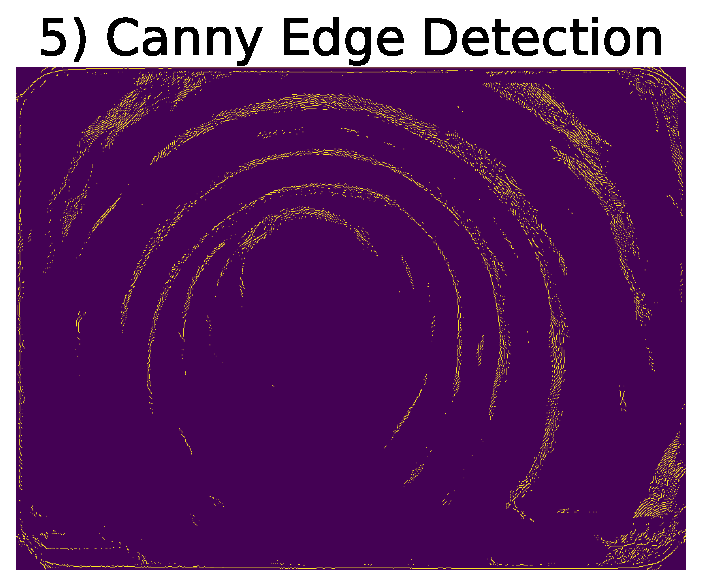
\includegraphics[width=\textwidth]{images/06_trach_cv/05_canny_edge_detection.pdf}};
    \end{tikzpicture}
    \begin{tikzpicture}
        \node[anchor=south west,inner sep=0] (image) at (0,0) {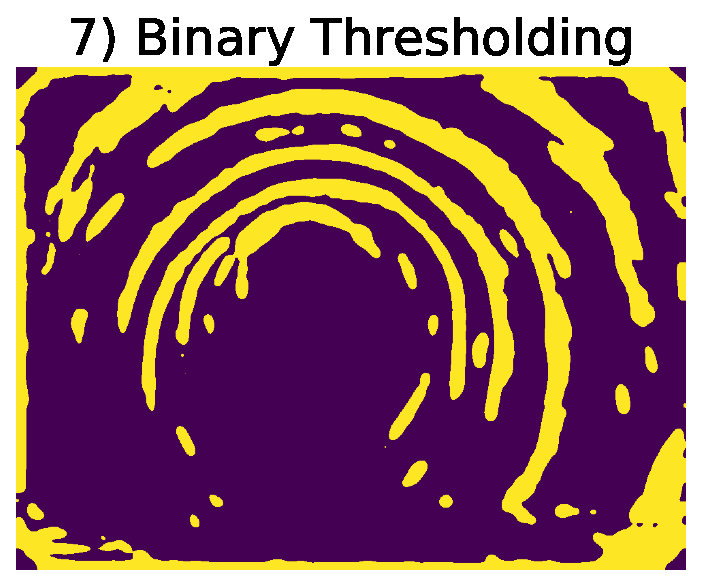
\includegraphics[width=\textwidth]{images/06_trach_cv/07_binary_thresholding.pdf}};
    \end{tikzpicture}
    \begin{tikzpicture}
        \node[anchor=south west,inner sep=0] (image) at (0,0) {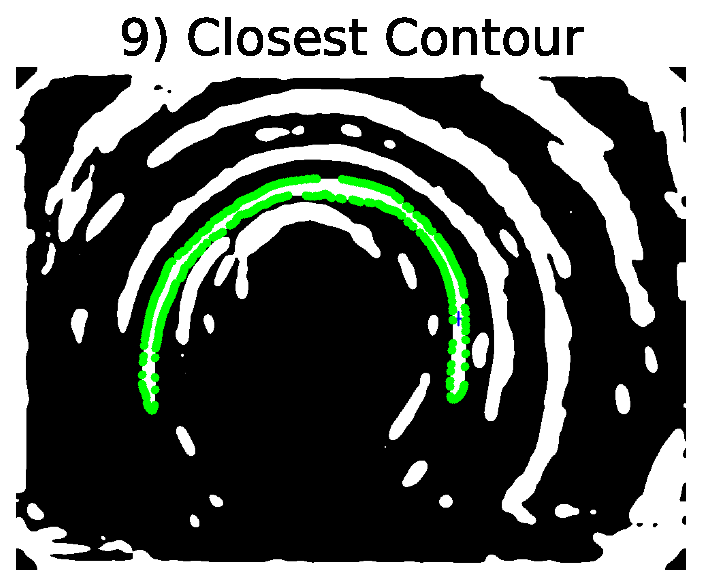
\includegraphics[width=\textwidth]{images/06_trach_cv/09_closest_contour.pdf}};
    \end{tikzpicture}
\end{minipage}
\hfill % Minimal space between columns
\begin{minipage}[t]{0.48\columnwidth} % Right column
    \centering
    \begin{tikzpicture}
        \node[anchor=south west,inner sep=0] (image) at (0,0) {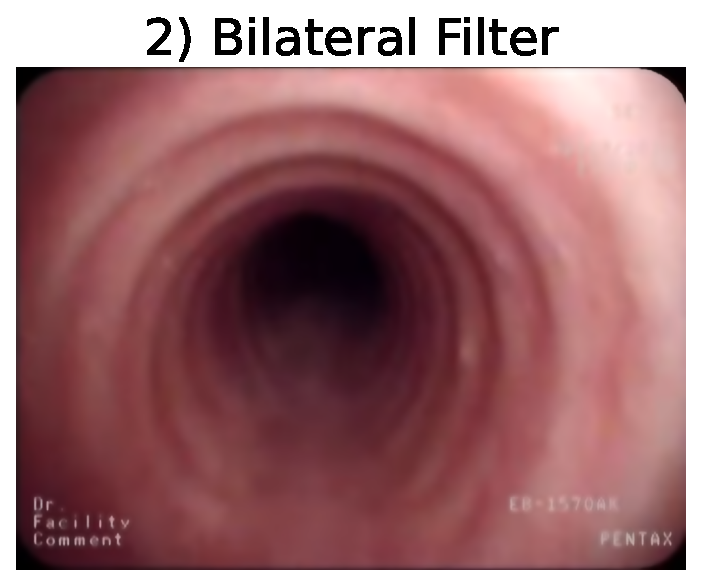
\includegraphics[width=\textwidth]{images/06_trach_cv/02_bilateral_filter.pdf}};
    \end{tikzpicture}
    \begin{tikzpicture}
        \node[anchor=south west,inner sep=0] (image) at (0,0) {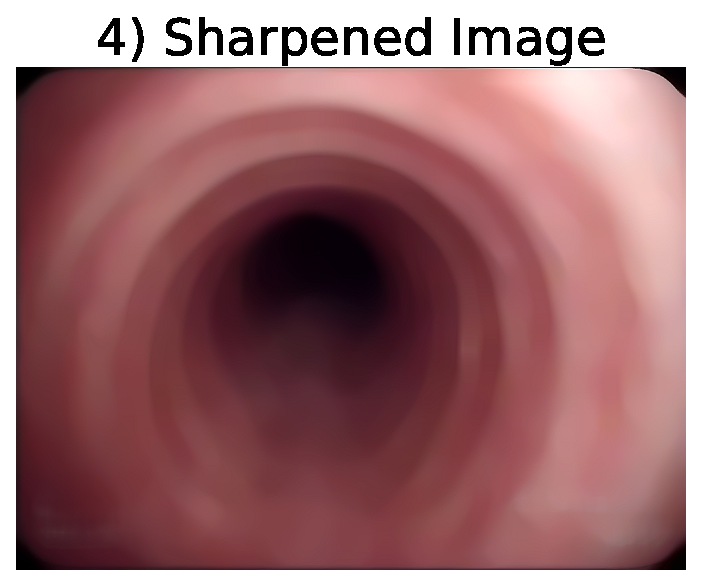
\includegraphics[width=\textwidth]{images/06_trach_cv/04_sharpened_image.pdf}};
    \end{tikzpicture}
    \begin{tikzpicture}
        \node[anchor=south west,inner sep=0] (image) at (0,0) {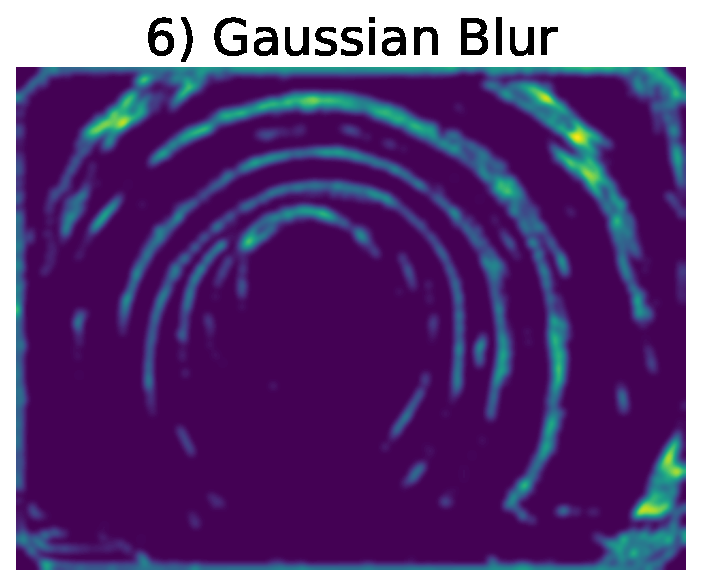
\includegraphics[width=\textwidth]{images/06_trach_cv/06_gaussian_blur.pdf}};
    \end{tikzpicture}
    \begin{tikzpicture}
        \node[anchor=south west,inner sep=0] (image) at (0,0) {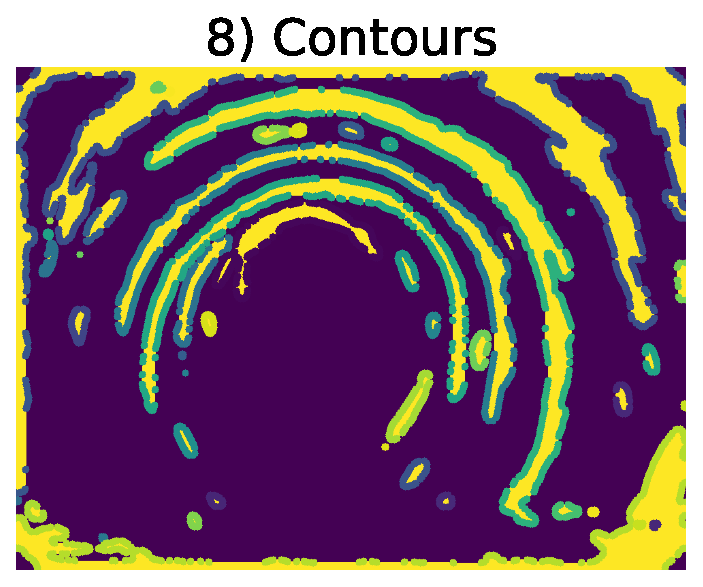
\includegraphics[width=\textwidth]{images/06_trach_cv/08_contours.pdf}};
    \end{tikzpicture}
    \begin{tikzpicture}
        \node[anchor=south west,inner sep=0] (image) at (0,0) {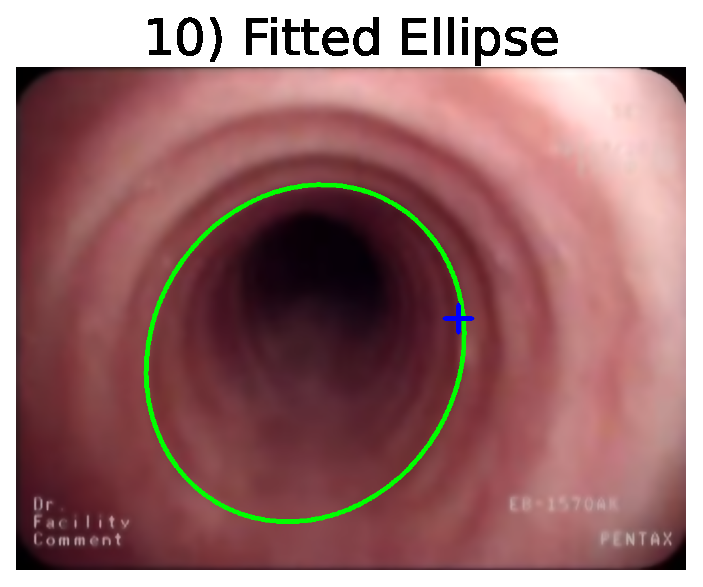
\includegraphics[width=\textwidth]{images/06_trach_cv/10_fitted_ellipse.pdf}};
    \end{tikzpicture}
\end{minipage}
\caption{Image processing pipeline for trachea analysis: 1) Source image, 2) Bilateral filter, 3) Median blur, 4) Sharpened image, 5) Canny edge detection, 6) Gaussian blur, 7) Binary thresholding, 8) Contours, 9) Closest contour, 10) Fitted ellipse.}
\label{fig:image_processing_grid}
\end{figure}

\subsection{Results and Conclusion}

The CV pipeline successfully detected C-shaped tracheal cartilages in the selected real VB image, demonstrating the feasibility of computer vision for identifying anatomical landmarks. In this experiment, the probe tip’s location was manually specified at an arbitrary point in the image, serving as a reference for contour selection. This approach could potentially integrate with the dimension estimation method described in Section \ref{sec:cv_meta_analysis}, providing a shape-detection component for airway measurement.

While the pipeline yielded promising results for the carefully selected image, its applicability in clinical scenarios is constrained by several factors. Real-world VB footage often involves camera misalignment (e.g., tilting or off-center positioning) and degraded image quality due to blood, mucus, or motion artifacts. Additionally, tracheal deformities, as exemplified in Figure \ref{fig:scene01123}, produce irregular cross-sectional shapes that may not be adequately approximated by an elliptical fit. These challenges highlight the need for further refinement to ensure robustness under typical clinical conditions.

\begin{figure}[h]
  \centering
  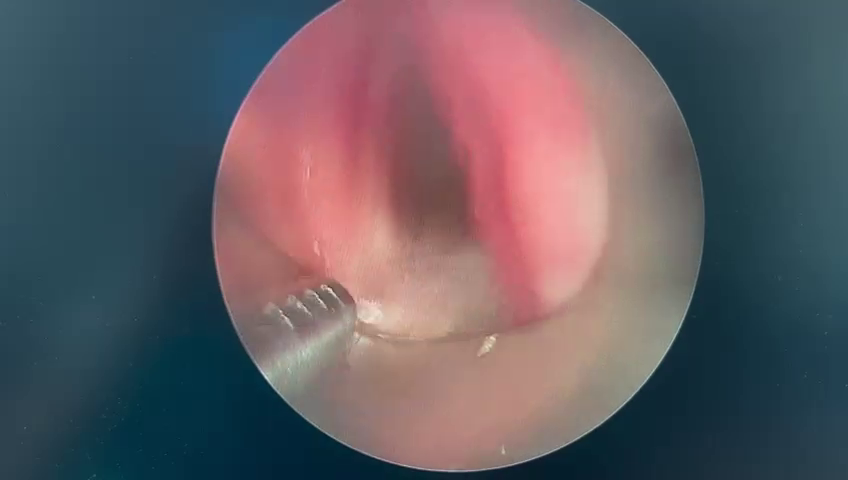
\includegraphics[width=1\columnwidth]{images/06_trach_cv/scene01123.png}
  \caption{Blurry VB image of a trachea with deformed geometry, illustrating conditions likely unsuitable for the CV pipeline.}
  \label{fig:scene01123}
\end{figure}

%--------------------------------------------------------
%--------------------------------------------------------
%--------------------------------------------------------
%--------------------------------------------------------

\section{Annotation GUI Applications for Airway Dimension Estimation}

During the course of this project, authentic video bronchoscopy (VB) footage was obtained from the collaborating hospital, revealing the significant challenges associated with clinical scenarios in advanced lung cancer. The footage frequently exhibited poor image quality, primarily due to blood and mucus obstructing the camera lens or interfering with its autofocus mechanism, compounded by subtle movements of the bronchoscope head that are difficult to stabilize. These factors resulted in only brief segments of usable footage, severely limiting the feasibility of automated tool detection. Notably, contact between the biopsy forceps and the airway wall often caused blood to obscure the tool, further hindering automated analysis.

Given these constraints, this study shifted focus to a manual annotation approach to facilitate airway dimension estimation. This approach involves user-guided identification of key regions in the image, specifically the location and scale of the probe (e.g., biopsy forceps) and the shape and position of the airway cross-section.

\subsection{Polygon Dimension Estimator}

The Polygon Dimension Estimator is a PyQt5-based application, comprising approximately 350 lines of code, designed to support accurate airway dimension estimation by leveraging manual annotations. The application requires input images where the probe is positioned at the same distance from the camera as the target cross-section, minimizing scale-related errors. A key feature is the ability to define arbitrary cross-sectional shapes through user-placed contiguous points, forming a polygon that represents the airway perimeter. The annotation backend adheres to object-oriented programming principles, though its design prioritizes functionality over extensibility. A representative screenshot of the application is shown in Figure \ref{fig:annotated_polygon}. The primary features include:

\begin{itemize}
    \item \textbf{Probe Calibration}: Utilizes the known diameter of the probe to compute a pixel-to-millimeter scale ratio, enabling accurate real-world measurements.
    \item \textbf{User-Defined Polygon}: Allows users to delineate complex cross-sectional geometries by specifying a series of contiguous points along the shape’s perimeter.
    \item \textbf{Ellipse Annotation}: Supports the placement of adjustable ellipses to mark the probe’s tip, with draggable handles for precise resizing, facilitating scale calibration.
    \item \textbf{Dimension and Area Calculation}: Computes the width and height (in millimeters) of the polygon’s bounding box and its area (in square millimeters) using OpenCV, based on the calibrated scale.
    \item \textbf{Interactive Interface}: Provides functionality for loading images (PNG, JPG, BMP), toggling polygon editing modes, clearing annotations, inputting probe diameter, and displaying results (scale, dimensions, area).
    \item \textbf{Dynamic Scaling}: Adjusts the displayed image to fit the window size while maintaining annotation accuracy in the original coordinate system.
    \item \textbf{Input Validation}: Incorporates error handling to alert users if polygons have fewer than three points or if scale calibration fails.
\end{itemize}

\begin{figure}[h]
  \centering
  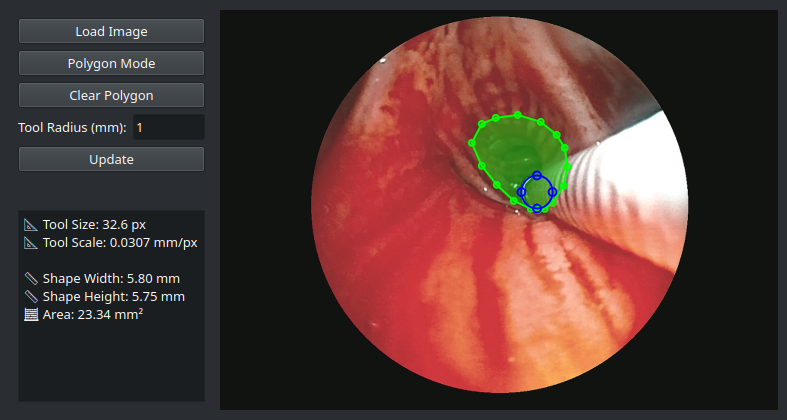
\includegraphics[width=1\columnwidth]{images/07_app/annotated_polygon.png}
  \caption{Screenshot of the Polygon Dimension Estimator application, with the probe radius set to 1 mm, an in-image probe size of 32.2 pixels, and an estimated polygon bounding box of 5.8 mm in height and 5.75 mm in width.}
  \label{fig:annotated_polygon}
\end{figure}

\subsection{Virtual Probe Provider}

The Virtual Probe Provider is a PyQt5-based application, comprising approximately 1,000 lines of code, designed to calibrate and visualize cylindrical probes in VB images. It offers a robust platform for manual probe annotation and cross-sectional dimension estimation. A screenshot demonstrating probe manipulation is shown in Figure \ref{fig:virt_probe_moved}. The primary features include:

\begin{itemize}
    \item \textbf{Reference Probe Definition}: Enables users to define a reference probe by placing two draggable lines on the image, with the probe’s position and orientation derived from their intersection and angle bisector, ensuring geometric precision.
    \item \textbf{3D Probe Visualization}: Renders probes as pseudo-3D cylinders, with customizable display options including skeleton outlines, filled bodies, measurement rulers, and an animated cursor for enhanced visual clarity.
    \item \textbf{Virtual Probe Adjustment}: Supports the creation of a virtual probe, which can be repositioned via a handle, with adjustable radius (0.01–15.00× multiplier), drawing limits, and cursor positioning for flexible analysis.
    \item \textbf{Interactive Controls}: Features sliders for radius scaling, limit adjustments, and cursor positioning, alongside checkboxes for toggling visualization options, enhancing user control.
    \item \textbf{Scale Calibration}: Allows input of the probe’s real diameter (default: 3 mm) to compute a pixel-to-millimeter ratio, supporting accurate dimension estimation.
    \item \textbf{Real-Time Rendering}: Updates annotations dynamically at 60 Hz, with smooth animations and anti-aliased graphics for a responsive user experience.
    \item \textbf{Mode Switching}: Facilitates toggling between a reference probe definition mode and a virtual probe manipulation mode, streamlining the workflow.
    \item \textbf{Input Validation}: Ensures reliable calculations by validating probe radius inputs and checking for non-parallel lines to prevent intersection errors.
    \item \textbf{Probe Repositioning}: Includes an experimental feature allowing the virtual probe to be moved within the image plane while maintaining parallel alignment with the camera view, though this functionality remains under development and may exhibit instability (Figure \ref{fig:virt_probe_moved}).
\end{itemize}

\begin{figure}[h]
  \centering
  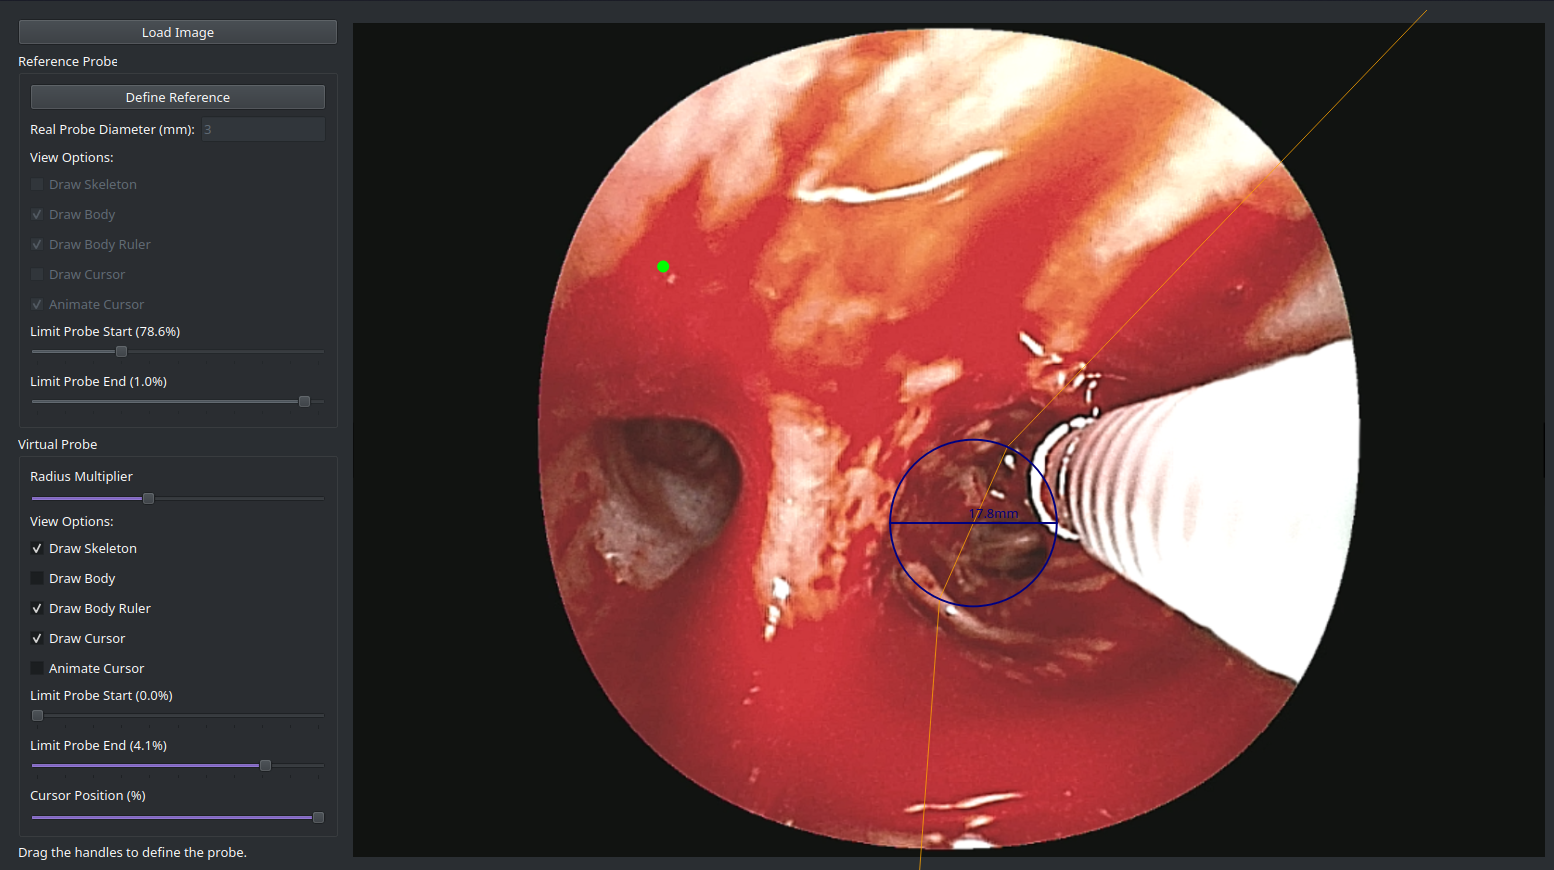
\includegraphics[width=1\columnwidth]{images/07_app/virt_probe_moved.png}
  \caption{Screenshot of the Virtual Probe Provider application, showing the virtual probe repositioned within the image plane while aligned parallel to the camera view.}
  \label{fig:virt_probe_moved}
\end{figure}

\subsubsection{Reference Probe Definition}
The users annotate the probe position and orientation in the image using two clickable lines. These lines define the probe’s geometry, which is mathematically transformed into a pseudo-3D cylindrical representation. The mathematical process for constructing this model is outlined below.

Two lines are defined by their endpoints, \( A_1, A_2 \) and \( B_1, B_2 \). The intersection point \( A \) is computed as the point where the lines meet, assuming they are not parallel. The direction vectors of the lines are normalized to unit vectors \( \mathbf{u}_1 \) and \( \mathbf{u}_2 \), respectively. The angle bisector direction is calculated as the normalized sum of these unit vectors:

\[
\mathbf{b} = \frac{\mathbf{u}_1 + \mathbf{u}_2}{\|\mathbf{u}_1 + \mathbf{u}_2\|}.
\]

A reference circle, approximating the probe’s base plane, is defined with a radius of 1.5 times the image width, based on empirical observations from reconstructing the camera-probe relationship in Blender. A point on the bisector, \( P_b \), is positioned at 90\% of this radius along the negative bisector direction from the intersection:

\[
P_b = A - \mathbf{b} \cdot 0.90 \cdot 1.5 \cdot \text{image width}.
\]

Similarly, a point on the first line, \( P_a \), is placed at the same distance along the negative direction of \( \mathbf{u}_1 \):

\[
P_a = A - \mathbf{u}_1 \cdot 0.90 \cdot 1.5 \cdot \text{image width}.
\]

The reference probe radius is the distance between \( P_b \) and \( P_a \). The \texttt{Probe} object is then constructed, centered at \( P_b \), with a direction vector from \( P_b \) to \( A \) and the computed radius. This object is rendered as a pseudo-3D cylinder.


\subsubsection{User Workflow for Cross-Section Estimation}

The Virtual Probe Provider guides users through a structured process to estimate airway cross-sectional diameters. Users begin by loading a VB image via the graphical user interface. In reference probe definition mode, they annotate the probe’s position and orientation, as shown in Figure \ref{fig:ref_probe_definition}. The real probe diameter is then input to calibrate the pixel-to-millimeter scale. Switching to virtual probe mode (Figure \ref{fig:virt_probe_same}), users muve the virtual probe’s tip to the target cross-section location by a sliter on the side. By adjusting the radius multiplier slider, the virtual probe’s radius is scaled to match the cross-section, with the estimated diameter (in millimeters) displayed alongside the probe’s cursor, as depicted in Figure \ref{fig:virt_probe_scaled}.

\begin{figure}[h]
  \centering
  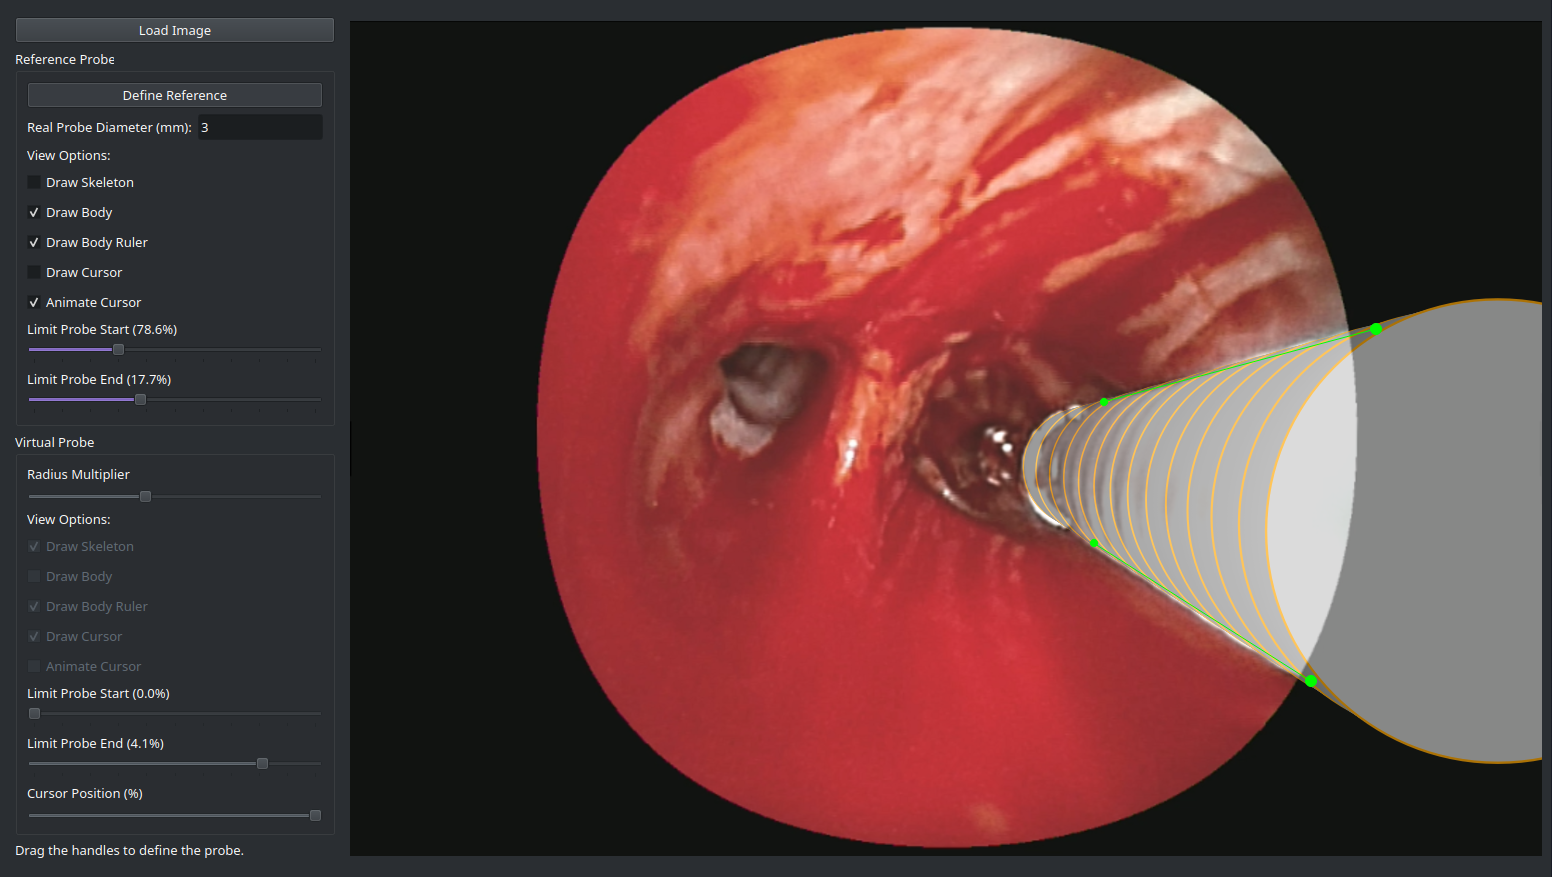
\includegraphics[width=1\columnwidth]{images/07_app/ref_probe_definition.png}
  \caption{Screenshot of the Virtual Probe Provider application, showing the reference probe being annotated.}
  \label{fig:ref_probe_definition}
\end{figure}

\begin{figure}[h]
  \centering
  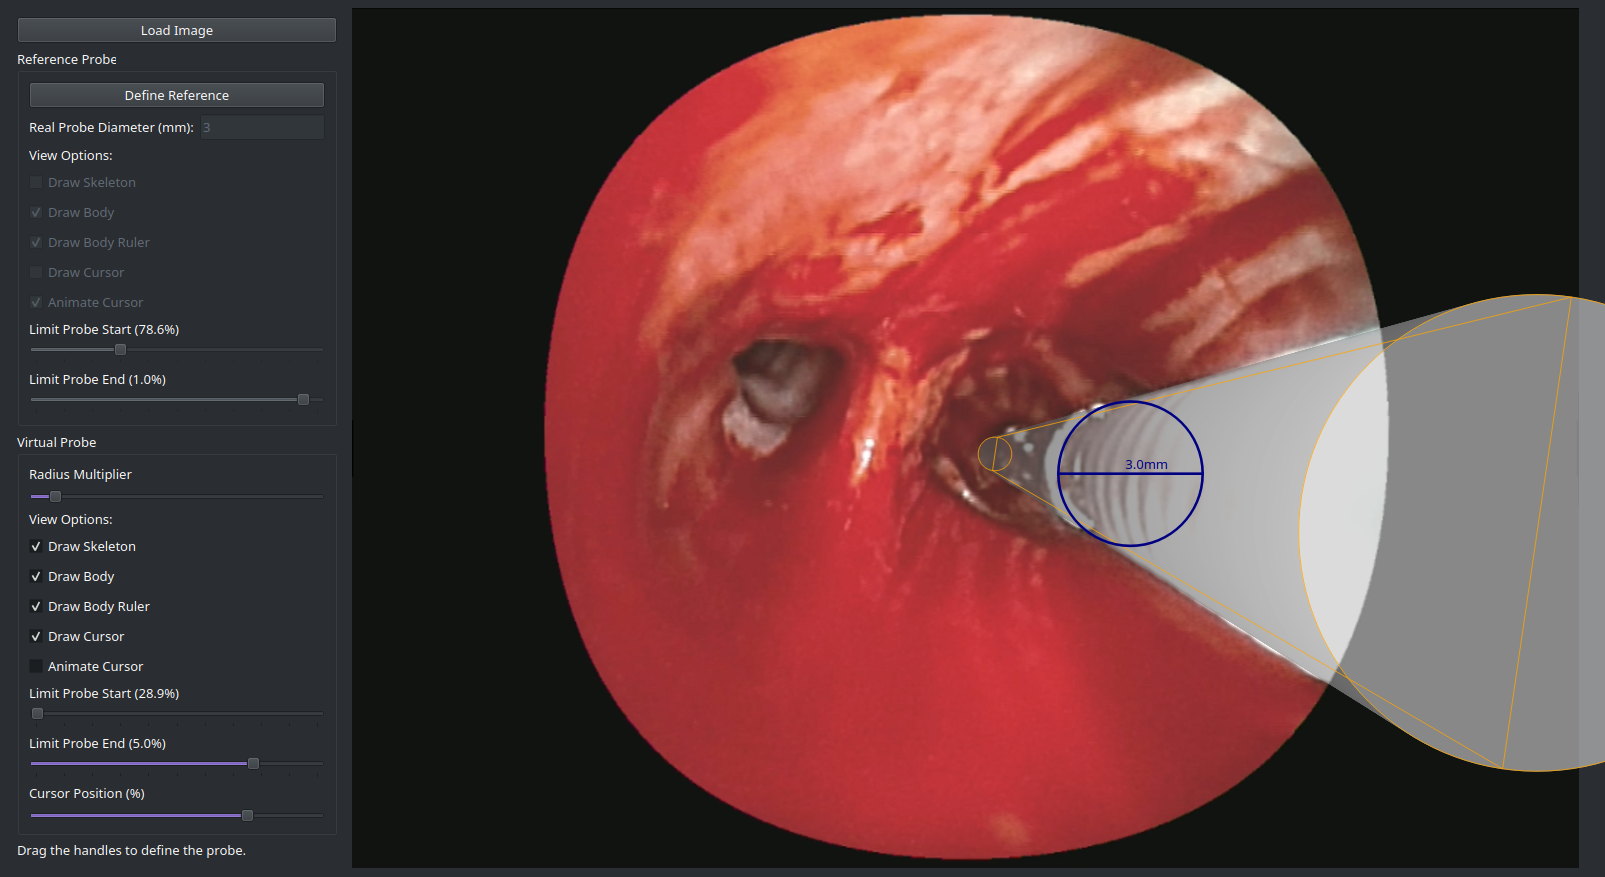
\includegraphics[width=1\columnwidth]{images/07_app/virt_probe_same.png}
  \caption{Screenshot of the Virtual Probe Provider application, transitioned to virtual probe mode.}
  \label{fig:virt_probe_same}
\end{figure}

\begin{figure}[h]
  \centering
  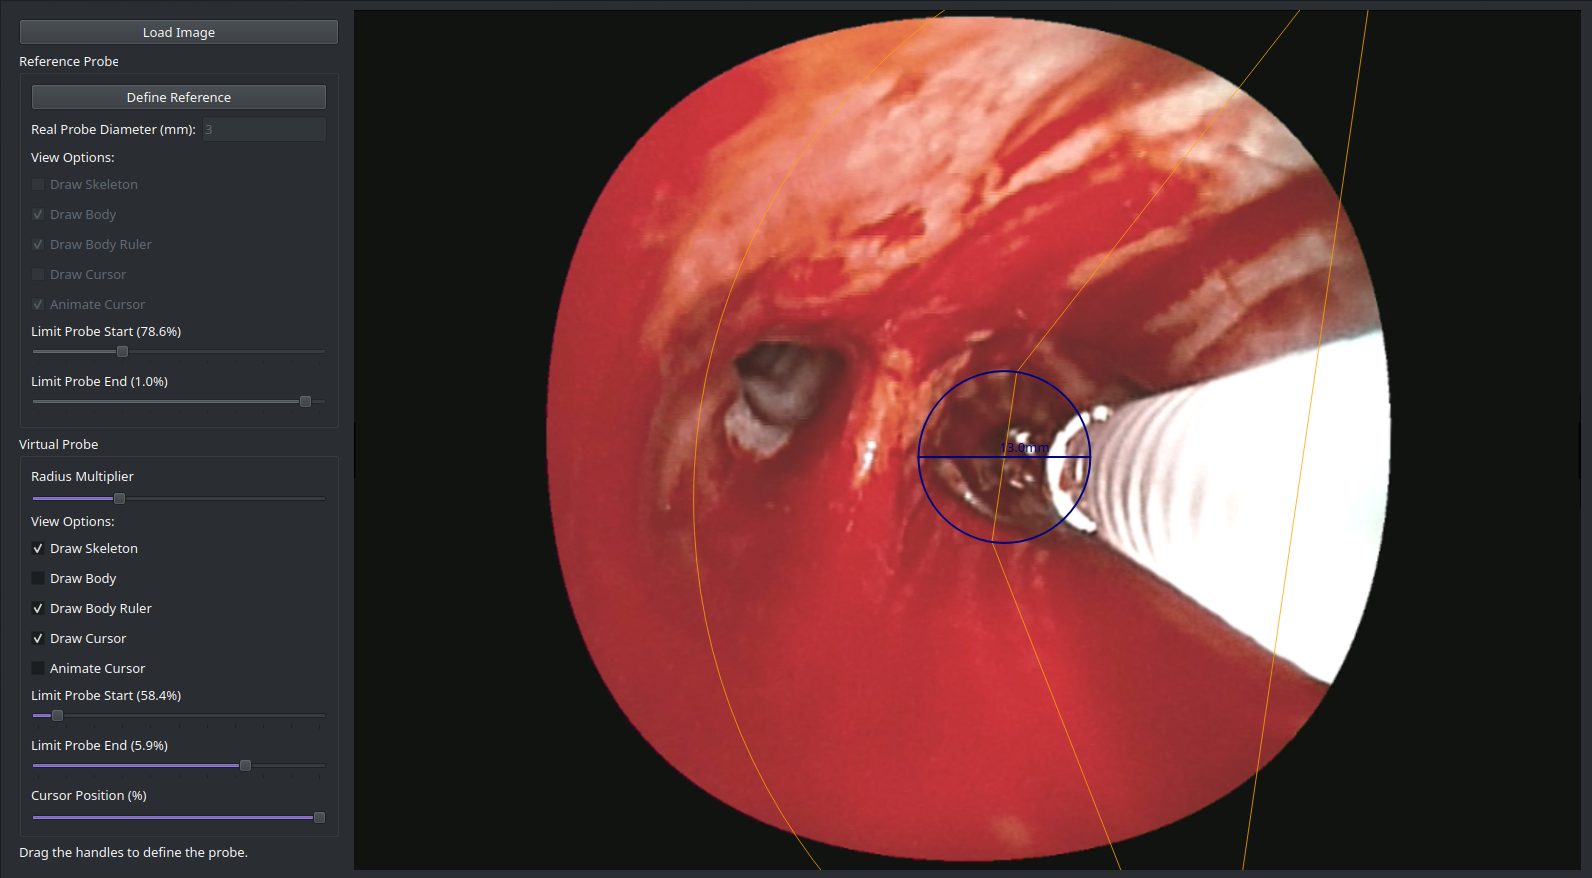
\includegraphics[width=1\columnwidth]{images/07_app/virt_probe_scaled.png}
  \caption{Screenshot of the Virtual Probe Provider application, with the virtual probe adjusted to align with the target cross-section and scaled to estimate its diameter.}
  \label{fig:virt_probe_scaled}
\end{figure}

\subsection{Conclusion}

The Polygon Dimension Estimator and Virtual Probe Provider applications can be used complementarily to analyze video bronchoscopy (VB) images that are unsuitable for automated processing, such as those exhibiting severe blur or obstructions from blood and mucus. For instance, an image where the probe is not ideally positioned at the target cross-section can be processed first in the Virtual Probe Provider to annotate or virtually extend the probe’s position to align with the desired cross-section. The resulting annotated image can then be loaded into the Polygon Dimension Estimator to manually define the target cross-sectional shape, accommodating non-circular geometries, and compute its dimensions (e.g., Figure \ref{fig:scene_poly_guess}).

Integrating the features of both applications into a single platform could enhance usability. Potential enhancements include support for video stream inputs, savable configurations, and automated probe detection to reduce manual effort.

These applications demonstrate the potential of user-guided, machine-aided methods to improve the assessment of airway stenosis severity from VB footage in advanced lung cancer. While currently reliant on manual annotations, they provide a practical framework for addressing the challenges of poor-quality clinical footage, laying the groundwork for future development toward more automated solutions.

\begin{figure}[h]
  \centering
  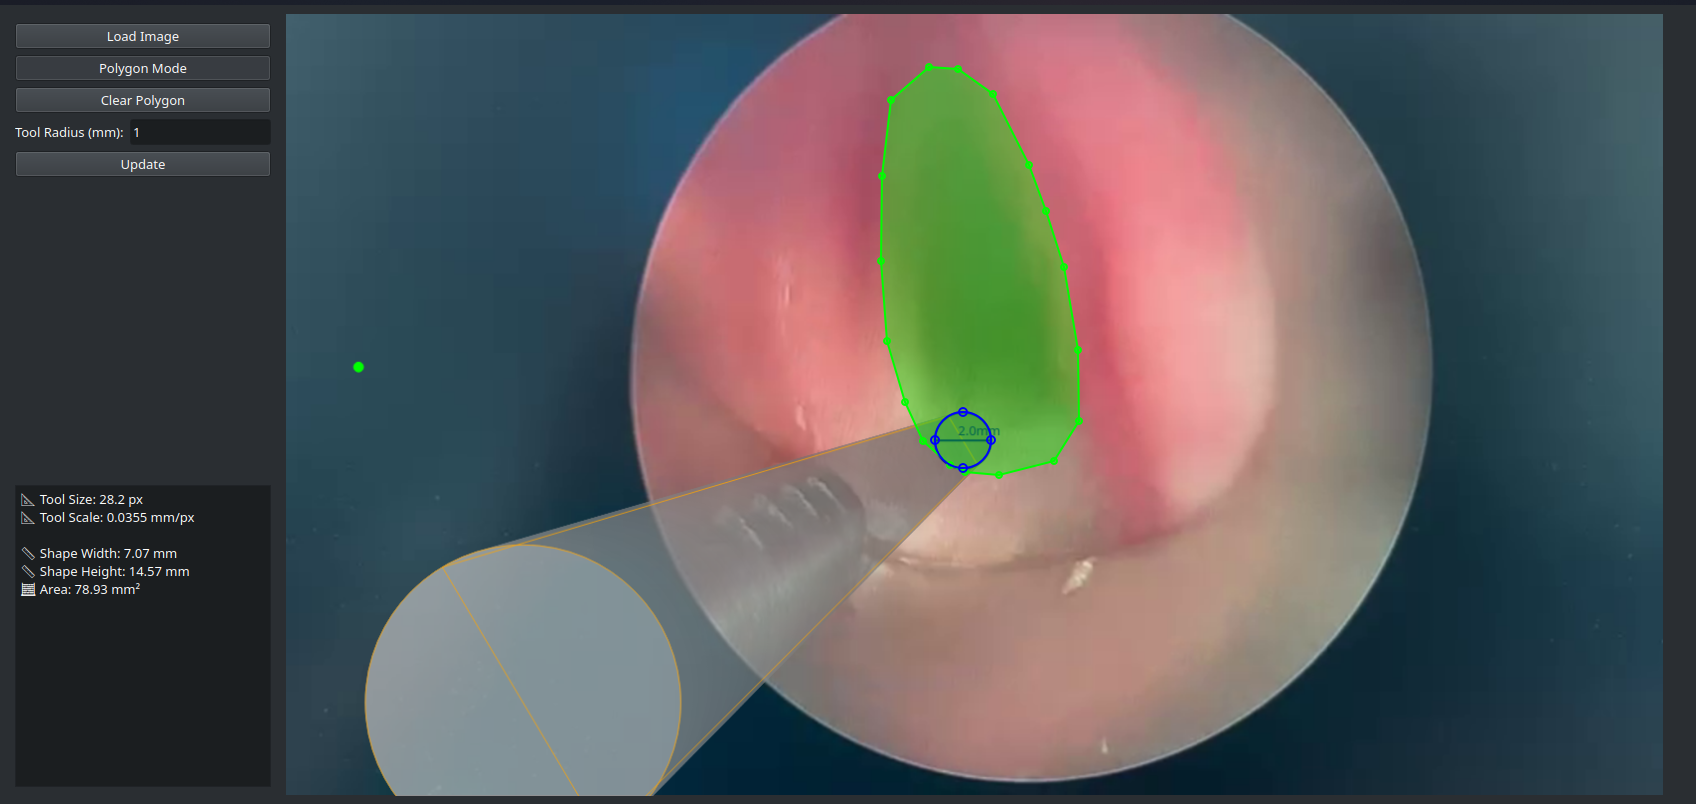
\includegraphics[width=1\columnwidth]{images/07_app/scene_poly_guess.png}
  \caption{Screenshot of the Polygon Dimension Estimator application, processing an image with an annotated cross-sectional polygon derived from a virtual probe adjustment.}
  \label{fig:scene_poly_guess}
\end{figure}


%--------------------------------------------------------
%--------------------------------------------------------
%--------------------------------------------------------
%--------------------------------------------------------
\section{Conclusions}
\label{sec:Conclusions}

My work focused on developing methods to estimate airway dimensions from VB footage for accurate airway stent sizing, addressing the lack of scale references in clinical images. We proposed using a rigid probe (e.g., biopsy forceps) with known dimensions as a scale reference. I then tested this approach through controlled 3D experiments, and extended it to realistic tracheal models and real VB images. Due to poor image quality and obstructions in clinical footage, which hindered automated detection, I developed two GUI applications (the Polygon Dimension Estimator and Virtual Probe Provider) to enable manual annotations for dimension estimation. The reader should remember that this work offers practical solutions for handling suboptimal VB footage, emphasizing manual annotation as a viable strategy when automation fails, and lays groundwork for future advancements in airway measurement.

The simplified 3D tube experiment demonstrated promising accuracy, with all diameter predictions within 1 mm of actual values, achieving a mean error of 0.451 mm, a median error of 0.437 mm, and a maximum error of 0.821 mm across 20 images. The CV pipeline successfully detected C-shaped tracheal cartilages in a real VB image. The GUI applications enabled precise manual annotations, with the Polygon Dimension Estimator computing cross-sectional dimensions (e.g., 5.8 mm height, 5.75 mm width for a sample polygon) and the Virtual Probe Provider facilitating probe repositioning and scale calibration. These results underscore the work’s significance in providing approximate yet actionable measurements under challenging clinical conditions.

The original contributions of this work include: (1) a probe-based methodology for airway dimension estimation, validated through controlled 3D experiments, offering a practical approach to scale calibration in VB footage; (2) the development of two PyQt5-based GUI applications that enable user-guided dimension estimation, addressing the limitations of automated methods in poor-quality clinical images; and (3) a proof-of-concept CV pipeline for detecting tracheal cartilages, highlighting both its potential and constraints in realistic scenarios. These contributions provide researchers and clinicians with tools and insights for tackling airway stent sizing in advanced lung cancer cases, emphasizing adaptability to suboptimal data.

Other researchers can build on this work by refining the CV pipeline to handle irregular cross-sections and mitigate lighting artifacts, potentially integrating machine learning for robust contour detection. The GUI applications could be enhanced with video stream support, automated probe detection, or integration into a single platform, improving usability in clinical settings. Developers might explore dynamic pixel-to-millimeter ratio calculations in 3D environments to eliminate empirical fitting functions.

\section*{Acknowledgements}
I would like to thank my supervisor Ing. Tomáš Goldmann, Ph.D. for his help and consultations.